\documentclass[10pt,
               xcolor={usenames,dvipsnames},
               hyperref={colorlinks,linktoc=all,citecolor=Plum,linkcolor=MidnightBlue,urlcolor=MidnightBlue},noamssymb]{beamer}
% FONTS
\usepackage[T1]{fontenc}
\usepackage{tgtermes}
\usepackage{amsmath}

% Font choice 2:
\usepackage[scaled=0.92]{PTSans}
\usepackage{amssymb}
\newcommand{\mathbold}[1]{\ensuremath{\boldsymbol{\mathbf{#1}}}}
\newcommand{\mbf}[1]{\ensuremath{\boldsymbol{\mathbf{#1}}}}

%\usefonttheme{professionalfonts}

\usepackage{scalefnt,letltxmacro}
\LetLtxMacro{\oldtextsc}{\textsc}
\renewcommand{\textsc}[1]{\oldtextsc{\fontfamily{lmr}\scalefont{1}#1}}

% \renewcommand*\ttdefault{lmvtt}
\usepackage[ttdefault=true]{AnonymousPro}

% GEOMETRY
%\usepackage[
%  paper  = letterpaper,
%  left   = 1.65in,
%  right  = 1.65in,
%  top    = 1.0in,
%  bottom = 1.0in,
%  ]{geometry}

% # COLOR

% \usepackage[usenames,dvipsnames]{xcolor}
\definecolor{shadecolor}{gray}{0.9}

% SPACING and TEXT
%\usepackage[final,expansion=alltext]{microtype}
\usepackage[english]{babel}
\usepackage[parfill]{parskip}
\usepackage{afterpage}
\usepackage{framed}
\usepackage{xspace}

% LEFTBAR
\renewenvironment{leftbar}[1][\hsize]
{%
  \def\FrameCommand
  {%
    {\color{Gray}\vrule width 3pt}%
    \hspace{10pt}%
    %\hspace{0pt}\fboxsep=\FrameSep\colorbox{black!10}%
  }%
  \MakeFramed{\hsize#1\advance\hsize-\width\FrameRestore}%
}%
{\endMakeFramed}

% EDITING
% line numbering in left margin
\usepackage{lineno}
\renewcommand\linenumberfont{\normalfont
                             \footnotesize
                             \sffamily
                             \color{SkyBlue}}
% ragged paragraphs in right margin
\usepackage{ragged2e}
% TODO should i rename sidenote marginpar?
\DeclareRobustCommand{\sidenote}[1]{\marginpar{
                                    \RaggedRight
                                    \textcolor{Plum}{\textsf{#1}}}}
% paragraph counter in right margin
\newcommand{\parnum}{\bfseries\P\arabic{parcount}}
\newcounter{parcount}
\newcommand\p{%
    \stepcounter{parcount}%
    \leavevmode\marginpar[\hfill\parnum]{\parnum}%
}
% pargraph header
\DeclareRobustCommand{\parhead}[1]{\textbf{#1}~}
% paragraph helper
\DeclareRobustCommand{\PP}{\textcolor{Plum}{\P} }

% COUNTERS
%\renewcommand{\labelenumi}{\color{black!67}{\arabic{enumi}.}}
%\renewcommand{\labelenumii}{{\color{black!67}(\alph{enumii})}}
%\renewcommand{\labelitemi}{{\color{black!67}\textbullet}}

% FIGURES
\usepackage{graphicx}
\usepackage[labelfont=bf]{caption}
%\usepackage[format=hang]{subcaption}

% TABLES
\usepackage{booktabs}
\usepackage{multirow}

% # ALGORITHMS

\usepackage[algoruled]{algorithm2e}
\setlength{\interspacetitleruled}{8pt}
\usepackage{listings}
\usepackage{fancyvrb}
\fvset{fontsize=\small}

% HYPERREF
%\usepackage[colorlinks,linktoc=all]{hyperref}
%\usepackage[all]{hypcap}
\hypersetup{citecolor=Plum}
\hypersetup{linkcolor=MidnightBlue}
\hypersetup{urlcolor=MidnightBlue}

% CLEVEREF must come after HYPERREF
\usepackage[nameinlink]{cleveref}
\newcommand{\Crefb}[1]{(\Cref{#1})}
\newcommand{\crefb}[1]{(\cref{#1})}

% ACRONYMS
\usepackage[acronym,smallcaps,nowarn]{glossaries}
\glsdisablehyper
% \makeglossaries

% COLOR DEFINITIONS
\newcommand{\red}[1]{\textcolor{BrickRed}{#1}}
\newcommand{\orange}[1]{\textcolor{BurntOrange}{#1}}
\newcommand{\green}[1]{\textcolor{OliveGreen}{#1}}
\newcommand{\blue}[1]{\textcolor{MidnightBlue}{#1}}
\newcommand{\gray}[1]{\textcolor{black!60}{#1}}

\newacronym{ELBO}{elbo}{evidence lower bound}
\newacronym{KL}{kl}{Kullback-Leibler}

\newacronym{DEF}{def}{deep exponential family}
\newacronym{DLGM}{dlgm}{deep latent Gaussian model}
\newacronym{DRAW}{draw}{Deep Recurrent Attentive Writer}

\newacronym{MF}{mf}{mean-field}
\newacronym{VGP}{vgp}{variational Gaussian process}
\newacronym{BBVI}{bbvi}{black box variational inference}
\newacronym{ADVI}{advi}{automatic differentiation variational inference}
\newacronym{NF}{nf}{normalizing flows}
\newacronym{CVI}{cvi}{copula variational inference}
\newacronym{VAE}{vae}{variational autoencoder}
\newacronym{IWAE}{iwae}{importance weighted autoencoder}
\newacronym{NVIL}{nvil}{neural variational inference}
\newacronym{MIXTURE}{mixture}{}
\newacronym{DSVI}{dsvi}{}

\newacronym{VI}{vi}{variational inference}
\newacronym{EP}{ep}{expectation propagation}

\newacronym{LS}{ls}{Langevin-Stein}
\newacronym{OPVI}{opvi}{operator variational inference}

% # PROBABILITY

\newcommand{\g}{\,|\,}
\renewcommand{\gg}{\,\|\,}
\DeclareRobustCommand{\KL}[2]{\ensuremath{\textrm{KL}\left(#1\;\|\;#2\right)}}

% # DISTRIBUTIONS

\newcommand{\Gam}{\textrm{Gam}}
\newcommand{\InvGam}{\textrm{InvGam}}

% # MISCELLANEOUS

\renewcommand{\d}[1]{\ensuremath{\operatorname{d}\!{#1}}}
\newcommand{\diag}{\textrm{diag}}
\newcommand{\supp}{\textrm{supp}}
\DeclareMathOperator*{\argmax}{arg\,max}
\DeclareMathOperator*{\argmin}{arg\,min}
\newcommand\indep{\protect\mathpalette{\protect\independenT}{\perp}}
\def\independenT#1#2{\mathrel{\rlap{$#1#2$}\mkern2mu{#1#2}}}

\newcommand{\E}{\mathbb{E}}
\newcommand{\Var}{\mathbb{V}\textrm{ar}}

\newcommand{\bbN}{\mathbb{N}}
\newcommand{\bbZ}{\mathbb{Z}}
\newcommand{\bbR}{\mathbb{R}}
\newcommand{\bbS}{\mathbb{S}}

\newcommand{\cG}{\mathcal{G}}
\newcommand{\cL}{\mathcal{L}}
\newcommand{\cF}{\mathcal{F}}
\newcommand{\cN}{\mathcal{N}}
\newcommand{\cQ}{\mathcal{Q}}

% # BOLD MATHEMATICS

\newcommand{\mba}{\mathbold{a}}
\newcommand{\mbb}{\mathbold{b}}
\newcommand{\mbc}{\mathbold{c}}
\newcommand{\mbd}{\mathbold{d}}
\newcommand{\mbe}{\mathbold{e}}
%\newcommand{\mbf}{\mathbold{f}}
\newcommand{\mbg}{\mathbold{g}}
\newcommand{\mbh}{\mathbold{h}}
\newcommand{\mbi}{\mathbold{i}}
\newcommand{\mbj}{\mathbold{j}}
\newcommand{\mbk}{\mathbold{k}}
\newcommand{\mbl}{\mathbold{l}}
\newcommand{\mbm}{\mathbold{m}}
\newcommand{\mbn}{\mathbold{n}}
\newcommand{\mbo}{\mathbold{o}}
\newcommand{\mbp}{\mathbold{p}}
\newcommand{\mbq}{\mathbold{q}}
\newcommand{\mbr}{\mathbold{r}}
\newcommand{\mbs}{\mathbold{s}}
\newcommand{\mbt}{\mathbold{t}}
\newcommand{\mbu}{\mathbold{u}}
\newcommand{\mbv}{\mathbold{v}}
\newcommand{\mbw}{\mathbold{w}}
\newcommand{\mbx}{\mathbold{x}}
\newcommand{\mby}{\mathbold{y}}
\newcommand{\mbz}{\mathbold{z}}

\newcommand{\mbA}{\mathbold{A}}
\newcommand{\mbB}{\mathbold{B}}
\newcommand{\mbC}{\mathbold{C}}
\newcommand{\mbD}{\mathbold{D}}
\newcommand{\mbE}{\mathbold{E}}
\newcommand{\mbF}{\mathbold{F}}
\newcommand{\mbG}{\mathbold{G}}
\newcommand{\mbH}{\mathbold{H}}
\newcommand{\mbI}{\mathbold{I}}
\newcommand{\mbJ}{\mathbold{J}}
\newcommand{\mbK}{\mathbold{K}}
\newcommand{\mbL}{\mathbold{L}}
\newcommand{\mbM}{\mathbold{M}}
\newcommand{\mbN}{\mathbold{N}}
\newcommand{\mbO}{\mathbold{O}}
\newcommand{\mbP}{\mathbold{P}}
\newcommand{\mbQ}{\mathbold{Q}}
\newcommand{\mbR}{\mathbold{R}}
\newcommand{\mbS}{\mathbold{S}}
\newcommand{\mbT}{\mathbold{T}}
\newcommand{\mbU}{\mathbold{U}}
\newcommand{\mbV}{\mathbold{V}}
\newcommand{\mbW}{\mathbold{W}}
\newcommand{\mbX}{\mathbold{X}}
\newcommand{\mbY}{\mathbold{Y}}
\newcommand{\mbZ}{\mathbold{Z}}

\newcommand{\mbalpha}{\mathbold{\alpha}}
\newcommand{\mbbeta}{\mathbold{\beta}}
\newcommand{\mbdelta}{\mathbold{\delta}}
\newcommand{\mbepsilon}{\mathbold{\epsilon}}
\newcommand{\mbchi}{\mathbold{\chi}}
\newcommand{\mbeta}{\mathbold{\eta}}
\newcommand{\mbgamma}{\mathbold{\gamma}}
\newcommand{\mbiota}{\mathbold{\iota}}
\newcommand{\mbkappa}{\mathbold{\kappa}}
\newcommand{\mblambda}{\mathbold{\lambda}}
\newcommand{\mbmu}{\mathbold{\mu}}
\newcommand{\mbnu}{\mathbold{\nu}}
\newcommand{\mbomega}{\mathbold{\omega}}
\newcommand{\mbphi}{\mathbold{\phi}}
\newcommand{\mbpi}{\mathbold{\pi}}
\newcommand{\mbpsi}{\mathbold{\psi}}
\newcommand{\mbrho}{\mathbold{\rho}}
\newcommand{\mbsigma}{\mathbold{\sigma}}
\newcommand{\mbtau}{\mathbold{\tau}}
\newcommand{\mbtheta}{\mathbold{\theta}}
\newcommand{\mbupsilon}{\mathbold{\upsilon}}
\newcommand{\mbvarepsilon}{\mathbold{\varepsilon}}
\newcommand{\mbvarphi}{\mathbold{\varphi}}
\newcommand{\mbvartheta}{\mathbold{\vartheta}}
\newcommand{\mbvarrho}{\mathbold{\varrho}}
\newcommand{\mbxi}{\mathbold{\xi}}
\newcommand{\mbzeta}{\mathbold{\zeta}}

\newcommand{\mbDelta}{\mathbold{\Delta}}
\newcommand{\mbGamma}{\mathbold{\Gamma}}
\newcommand{\mbLambda}{\mathbold{\Lambda}}
\newcommand{\mbOmega}{\mathbold{\Omega}}
\newcommand{\mbPhi}{\mathbold{\Phi}}
\newcommand{\mbPi}{\mathbold{\Pi}}
\newcommand{\mbPsi}{\mathbold{\Psi}}
\newcommand{\mbSigma}{\mathbold{\Sigma}}
\newcommand{\mbTheta}{\mathbold{\Theta}}
\newcommand{\mbUpsilon}{\mathbold{\Upsilon}}
\newcommand{\mbXi}{\mathbold{\Xi}}

\newcommand{\mbzero}{\mathbold{0}}
\newcommand{\mbone}{\mathbold{1}}
\newcommand{\mbtwo}{\mathbold{2}}
\newcommand{\mbthree}{\mathbold{3}}
\newcommand{\mbfour}{\mathbold{4}}
\newcommand{\mbfive}{\mathbold{5}}
\newcommand{\mbsix}{\mathbold{6}}
\newcommand{\mbseven}{\mathbold{7}}
\newcommand{\mbeight}{\mathbold{8}}
\newcommand{\mbnine}{\mathbold{9}}

\usepackage{tikz}
\usetikzlibrary{bayesnet}

\pgfdeclarelayer{edgelayer}
\pgfdeclarelayer{nodelayer}
\pgfsetlayers{edgelayer,nodelayer,main}

\definecolor{hexcolor0xbfbfbf}{rgb}{0.749,0.749,0.749}

\tikzset{>=latex}
\tikzstyle{none}   = [inner sep=0pt]

\tikzstyle{line}  = [ - ]
\tikzstyle{arrow}  = [ ->, shorten <=1pt, shorten >=1pt ]
\tikzstyle{ardash} = [ dotted, ->, shorten <=1pt, shorten >=1pt ]

\tikzstyle{empty}=[circle,opacity=0.0,text opacity=1.0,inner sep=0pt,minimum
width=0pt,minimum height=0pt]
\tikzstyle{box}=[rectangle,fill=White,draw=Black, inner sep=4pt]
\tikzstyle{filled}=[circle,fill=hexcolor0xbfbfbf,draw=Black]
\tikzstyle{hollow}=[circle,fill=White,draw=Black]
\tikzstyle{param}=[rectangle,fill=Black,draw=Black,inner sep=0pt,minimum width=4pt,minimum height=4pt]


\usepackage{subfigure}
\definecolor{light}{RGB}{199, 153, 199}
\definecolor{dark}{RGB}{143, 39, 143}
\definecolor{gray80}{gray}{0.8}

\usepackage{natbib}
\setbeamertemplate{navigation symbols}{}
\setbeamertemplate{itemize items}[circle]
\setbeamercolor{itemize item}{fg=black!67}
\setbeamercolor*{enumerate item}{fg=black!67}
\setbeamercolor*{enumerate subitem}{fg=black!67}
\setbeamercolor*{enumerate subsubitem}{fg=black!67}

\definecolor{charcoal}{HTML}{222222}
\definecolor{snow}{HTML}{F9F9F9}

\setbeamercolor{background canvas}{bg=white}
\setbeamercolor{normal text}{fg=charcoal}
\setbeamercolor{structure}{fg=charcoal}

\newenvironment{changemargin}[1]{
  \begin{list}{}{
    \setlength{\topsep}{0pt}
    \setlength{\leftmargin}{#1}
    \setlength{\rightmargin}{#1}
    \setlength{\listparindent}{\parindent}
    \setlength{\itemindent}{\parindent}
    \setlength{\parsep}{\parskip}
  }
  \item[]}{\end{list}}

\title{}
\begin{document}

\begin{frame}[plain,t]
\begin{tikzpicture}[remember picture,overlay]
  \node [xshift=0.50cm, yshift=-3.00cm, anchor=north west] at (current page.north west) {
    \begin{tabular}{l}
    {\Large\bf Everything You Didn't Know About Edward}\\[2ex]
    % {\Large\bf with Edward}\\[2ex]
    {\large }\\[4ex]
    Dustin Tran\\
    Columbia University \\[4ex]
    \end{tabular}
  };
  \node [xshift=-1.50cm, yshift=3.00cm, anchor=mid east] at (current page.south
  east) {
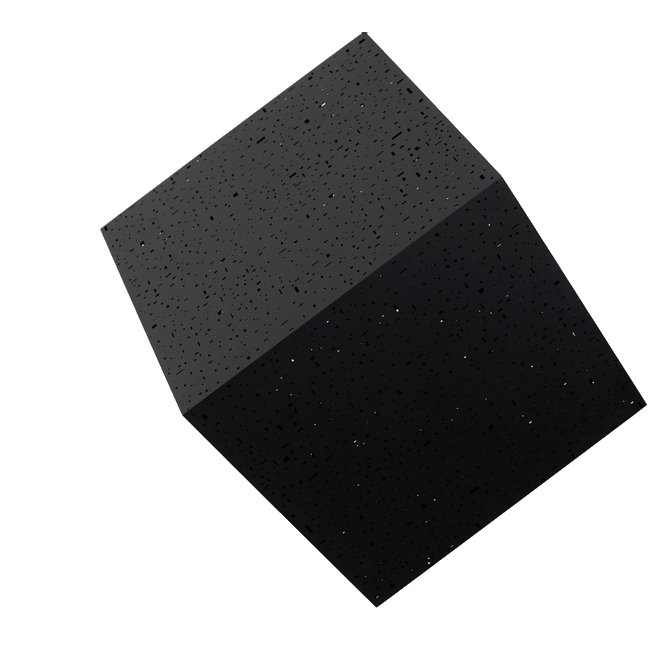
\includegraphics[width=0.25\textwidth]{img/edward.png}
  };
  % \node [xshift=-1.25cm, yshift=0.5cm, anchor=mid east] at (current page.south
  % east) {
  %   
\includegraphics[width=0.22\textwidth]{img/columbia.pdf}
  % };
  % \node [xshift=1.25cm, yshift=-0.9cm, anchor=mid east] at (current page.south
  % east) {
  %   
\includegraphics[width=0.40\textwidth]{img/openai.pdf}
  % };
\end{tikzpicture}
\end{frame}

\begin{frame}
\begin{center}
{\Large\bf Basics}
\end{center}
\end{frame}

\begin{frame}
\frametitle{What is probabilistic programming?}
\textbf{Probabilistic programs reify models from mathematics to
physical objects.}
\begin{itemize}
\vspace{-2ex}
\item
Each model is equipped with memory (``bits'',
floating point, storage) and computation
(``flops'', scalability, communication).
% from Gauss and Fisher to Turing and Church
\end{itemize}
\textbf{Anything you do lives in the world of probabilistic programming.}
\begin{itemize}
\item
Any computable model.

\gray{ex.
graphical models; neural networks; SVMs; stochastic processes.
}
\item
Any computable inference algorithm.

\gray{ex.
automated inference;
model-specific algorithms;
inference within inference (learning to learn).
}
\item
Any computable application.

\gray{ex.
exploratory analysis;
object recognition;
code generation;
causality.
}
\end{itemize}
\end{frame}

% \begin{frame}
% \begin{center}
% {\Huge
% \textit{\textbf{Simulation hypothesis.} \\
% ``The universe is a simulation from a computer program.''
% }
% \\[2ex]
% {\Large
% (Zuse, Bostrom, Schmidhuber, Musk)
% }}
% \end{center}
% % \vspace{3ex}
% % Probabilistic modeling is about positing a family of distribution and
% % finding the one true distribution.
% % \\[1ex]
% % Probabilistic programming is about finding the one true program.
% \end{frame}

% \begin{frame}
% \frametitle{George E.P. Box (1919 - 2013)}
% \begin{columns}
% \begin{column}{0.5\textwidth}
%     \begin{center}
%      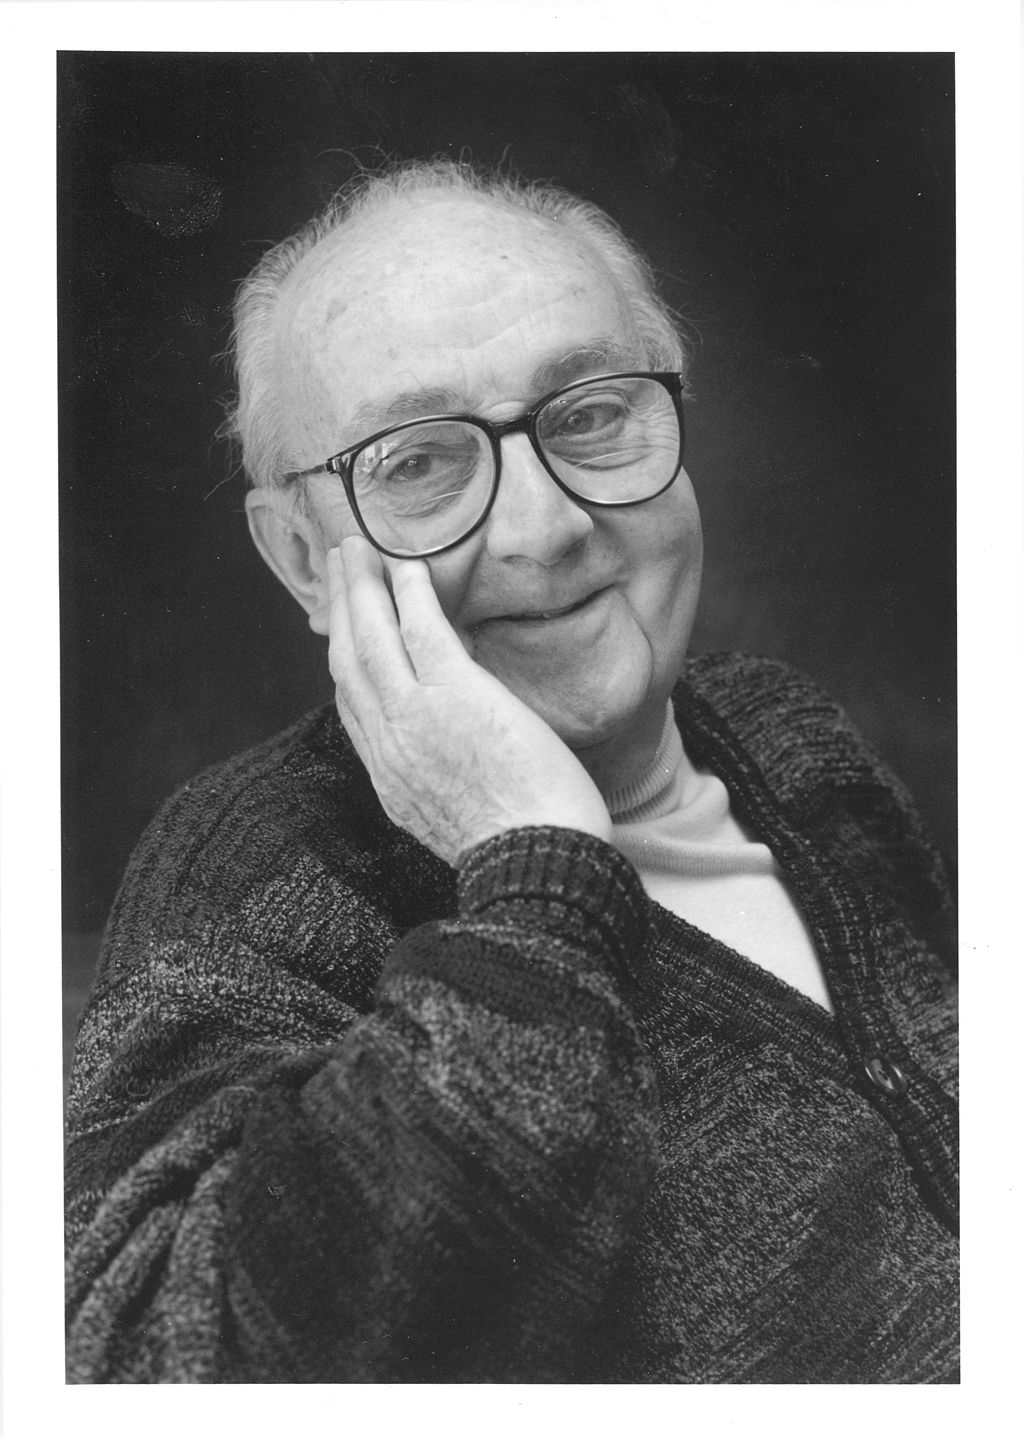
\includegraphics[width=\columnwidth]{img/box.jpg}
%      \end{center}
% \end{column}
% \begin{column}{0.5\textwidth}
% An iterative process for science:
% \\[1ex]
% \begin{enumerate}
% \item Build a model of the science
% \\[1ex]
% \item Infer the model given data
% \\[1ex]
% \item Criticize the model given data
% \end{enumerate}
% \end{column}
% \end{columns}
% \begin{tikzpicture}[remember picture,overlay]
%   \node [xshift=-8.0cm, yshift=0.4cm, anchor=south west] at (current
%   page.south east) {
% \gray{\small [Box \& Hunter 1962, 1965; Box \& Hill 1967; Box 1976, 1980]}
%   };
% \end{tikzpicture}
% \end{frame}

\begin{frame}
\frametitle{Box's Loop}
\begin{tikzpicture}[remember picture,overlay]
  \node [xshift=-1cm, yshift=-2.00cm, anchor=north west] at (current page.north west) {
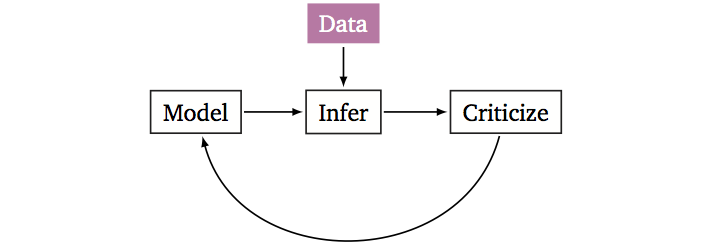
\includegraphics[width=1.4\textwidth]{img/model_infer_criticize.png}
  };
  \node [xshift=3.4cm, yshift=-8.0cm, anchor=north west] at (current page.north west) {
Edward is a library designed around this loop.
  };
  \node [xshift=0cm, yshift=-5.50cm, anchor=north west] at (current page.north west) {
  };
  \node [xshift=-4.0cm, yshift=0.4cm, anchor=south west] at (current
  page.south east) {
\gray{\small [Box 1976, 1980; Blei 2014]}
  };
\end{tikzpicture}
\end{frame}

% \begin{frame}
% \vspace{3ex}
% \textbf{Edward} is a probabilistic programming language
% built on TensorFlow.

% \emph{Modeling}
% \begin{itemize}
% \item
% Composable Turing-complete language of random variables.
% \item
% Many data types, tensor vectorization, broadcasting, 3rd party support.
% \item
% Examples:
% Graphical models, neural networks, Bayesian nonparametrics.
% \end{itemize}

% \emph{Inference}
% \begin{itemize}
% \item
% Composable language for hybrids, message passing, data subsampling.
% \item
% Infrastructure to develop your own algorithms.
% \item
% Examples:
% Black box VI, stochastic gradient MCMC, ABC.
% \end{itemize}

% \emph{Criticism}
% \begin{itemize}
% \item
% Examples: Scoring rules, hypothesis tests, predictive checks.
% \end{itemize}

% \vspace{1ex}
% Features include autodiff, multi-GPUs, distributed, XLA, quantization.

% \begin{tikzpicture}[remember picture,overlay]
%   \node [xshift=-3.0cm, yshift=0.4cm, anchor=south west] at (current
%   page.south east) {
% \gray{\small [Tran+ 2016, 2017]}
%   };
% \end{tikzpicture}
% \end{frame}

\begin{frame}
\begin{center}
\vspace{-2.5ex}
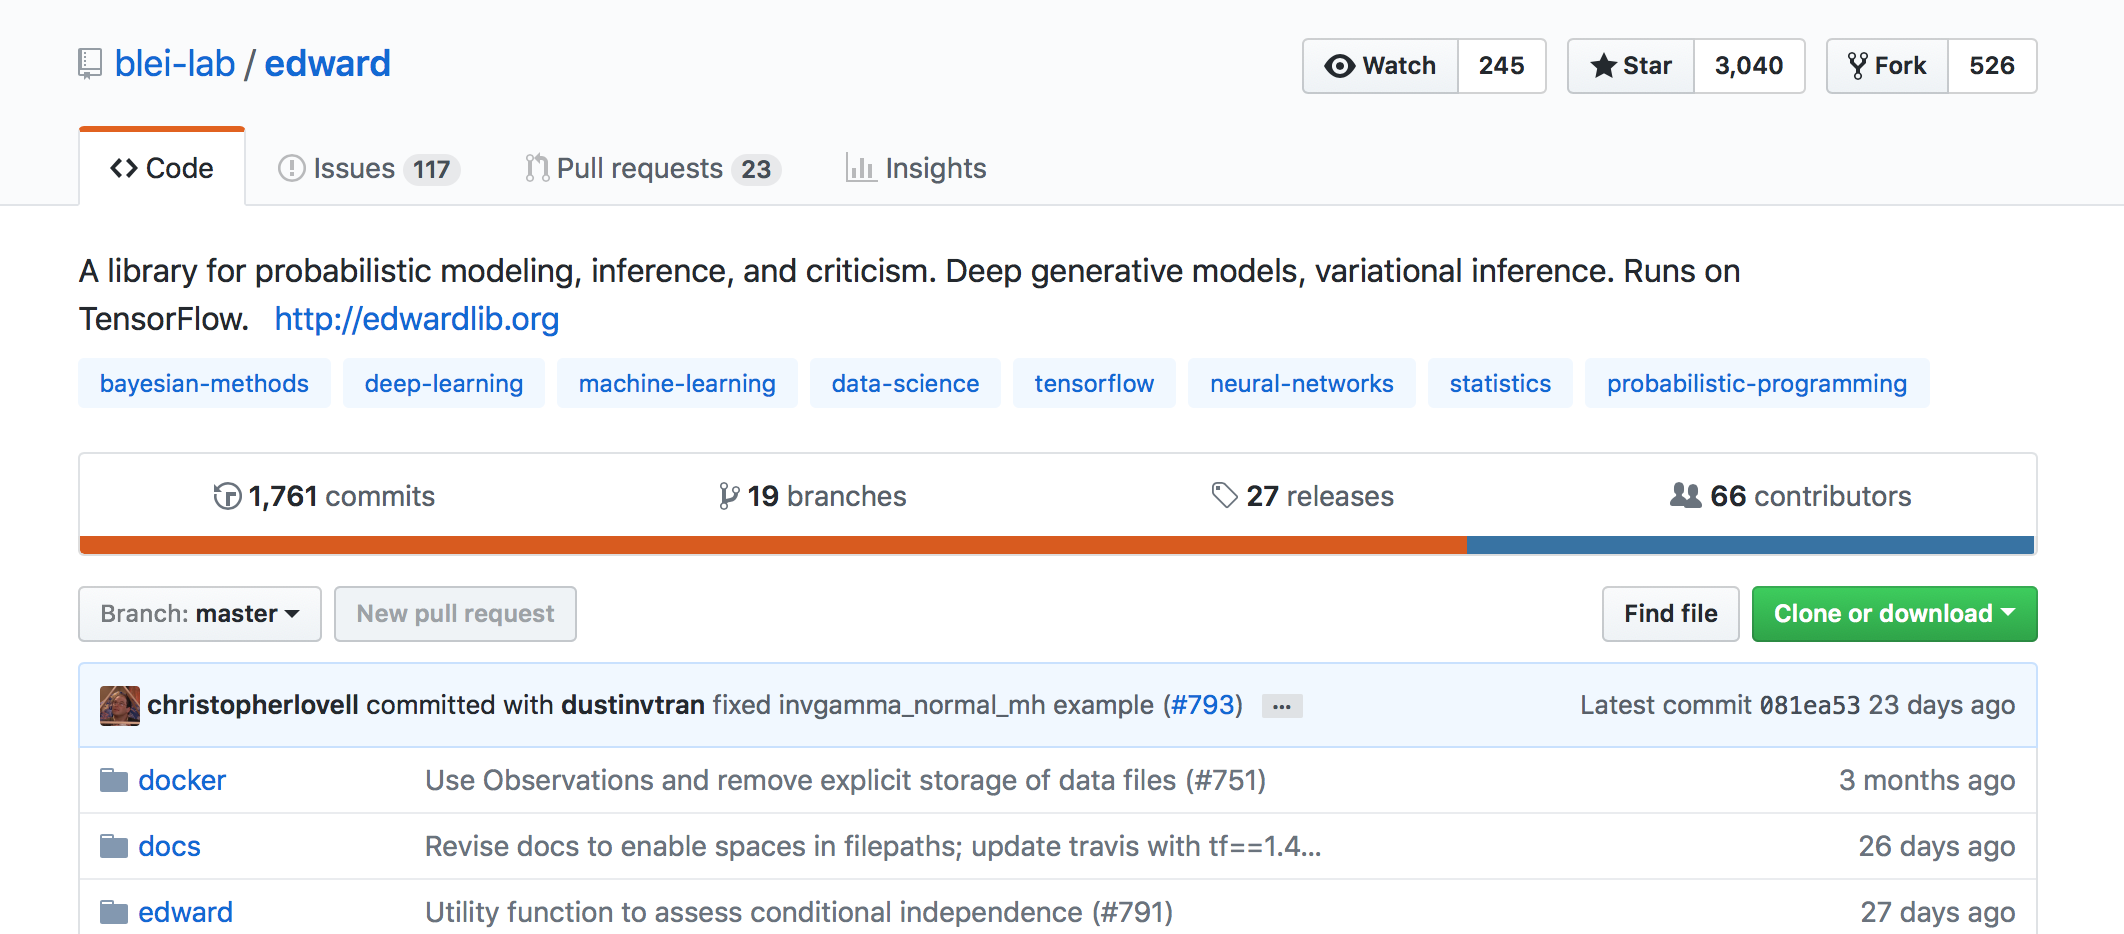
\includegraphics[width=1.0\textwidth]{img/github.png}
\\[-1.5ex]
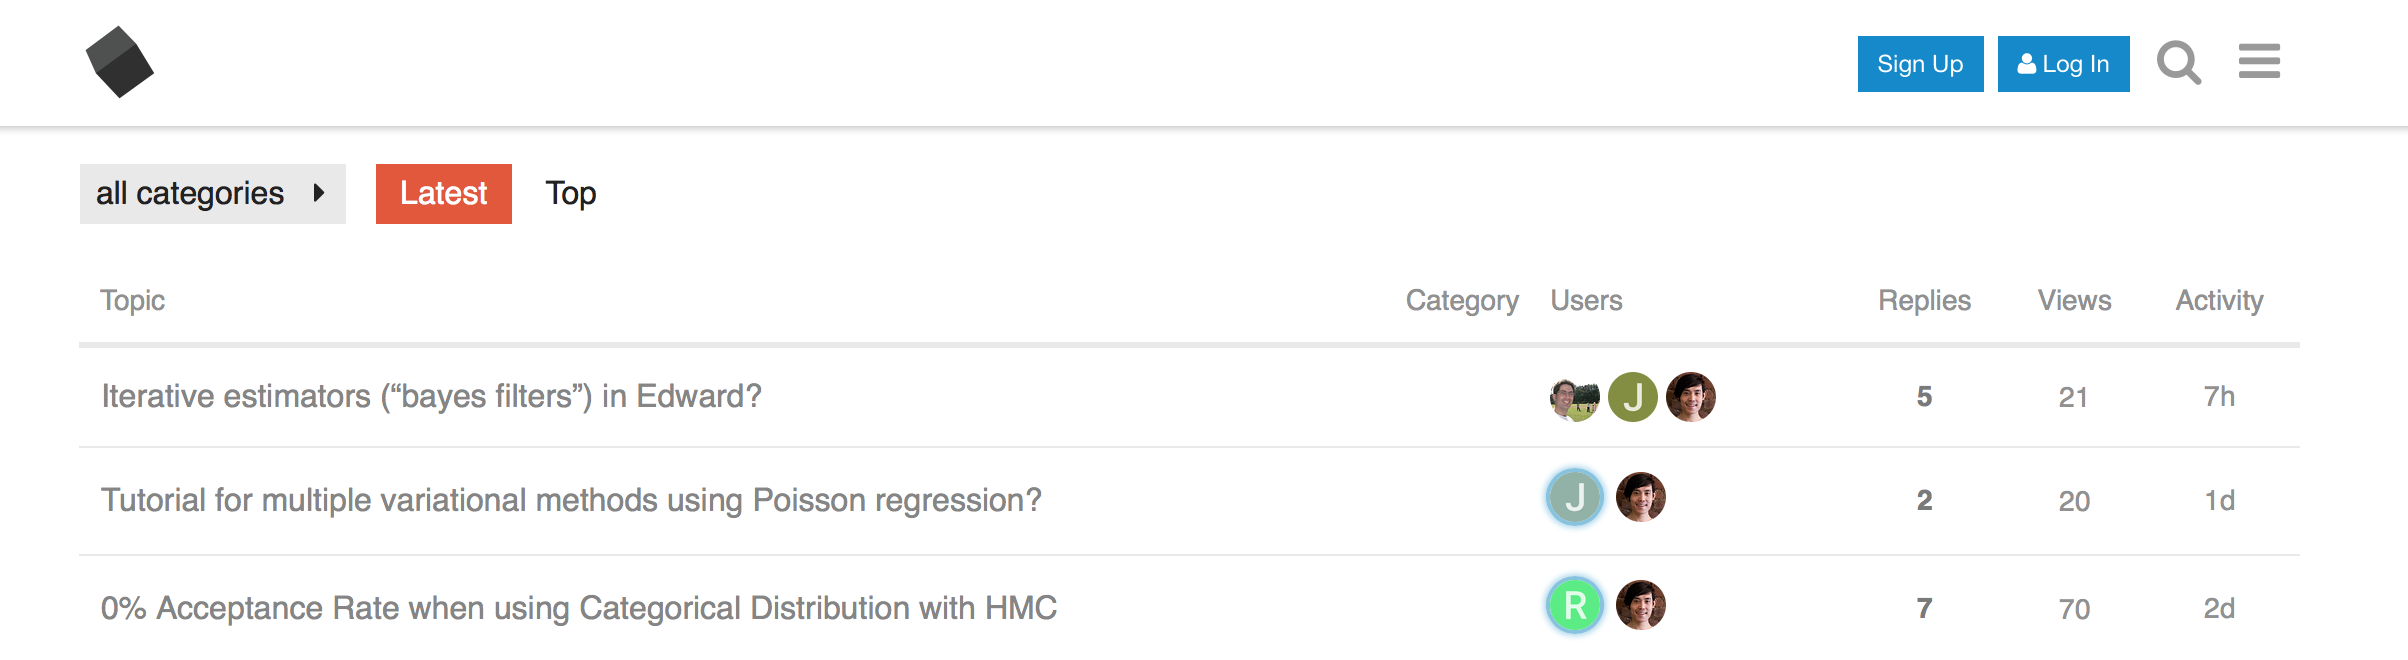
\includegraphics[width=1.0\textwidth]{img/forum.png}
\\[-3ex]
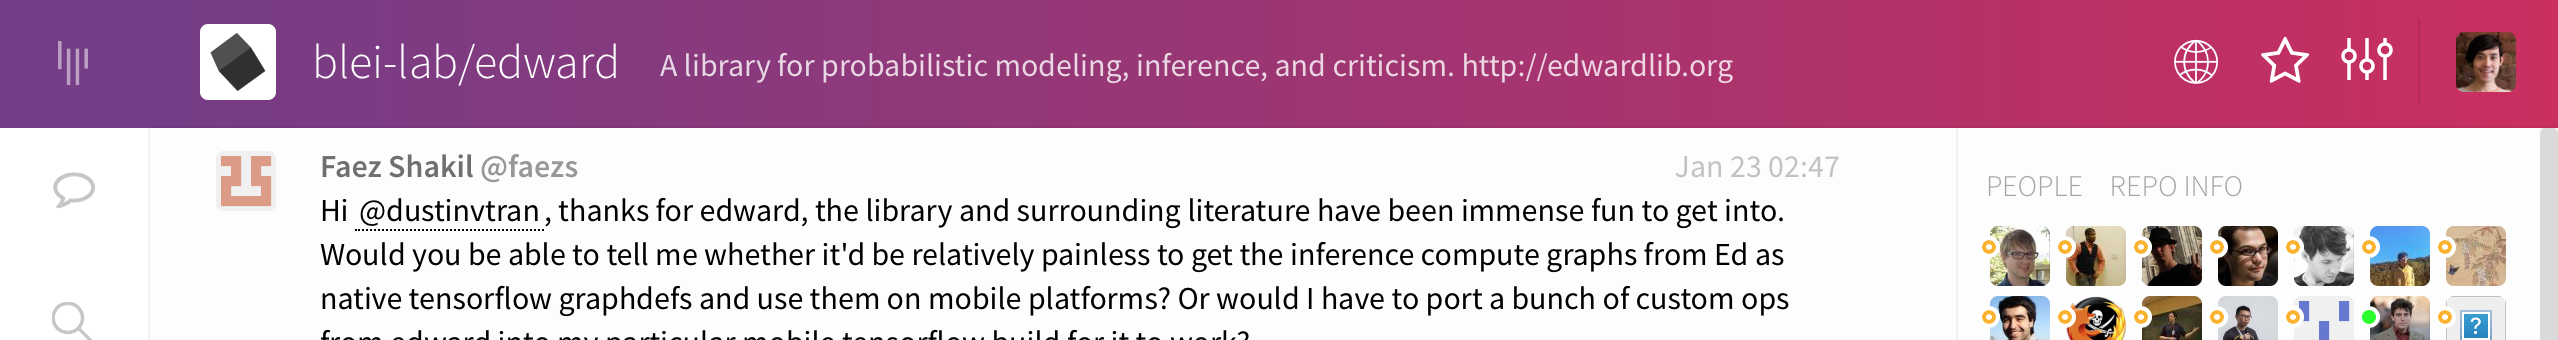
\includegraphics[width=1.0\textwidth]{img/gitter.png}
\\[2ex]
\end{center}
\text{
We have an active community of several thousand users \& many
contributors.
}
\end{frame}

\begin{frame}
\frametitle{What impact has Edward had?}
Designs
\begin{itemize}
\item
% \textbf{D.~Tran}, A.~Kucukelbir, A.~Dieng, M.~Rudolph, D.~Liang, and
% D.M.~Blei.
Edward: A library for probabilistic modeling, inference, and criticism.
\gray{arXiv, 2016.}
\item
% \textbf{D.~Tran}, M.D.~Hoffman, R.A.~Saurous, E.~Brevdo, K.~Murphy, and
% D.M.~Blei.
Deep probabilistic programming.
\gray{ICLR, 2017.}
\item
Book chapter.
\gray{arXiv next week, 2017.}
\end{itemize}

Applications
\begin{itemize}
\item
The variational Gaussian process.
\gray{ICLR, 2016.}
\item
Hierarchical variational models.
\gray{ICML, 2016.}
\item
Exponential family embeddings.
\gray{NIPS, 2016.}
\item
Deep and hierarchical implicit models.
\gray{NIPS, 2017.}
\item
Variational inference via $\chi$-upper bound minimization.
\gray{NIPS, 2017.}
\item
Causal effect inference with deep latent-variable models.
\gray{NIPS, 2017.}
\item
Implicit causal models for genome-wide association studies.
\gray{arXiv, 2017}
\item
% \textbf{D.~Tran} and D.M.~Blei. \\
Feature-matching auto-encoders.
\gray{OpenReview, 2017}
\end{itemize}
\end{frame}

% \begin{frame}
% \frametitle{Who is Using Edward?}
% {\large Users}
% \begin{enumerate}
% \item
% Machine learning enthusiasts, data scientists, business analysts \\
% (\emph{ex. hierarchical GLMs, mixture models, MAP, MCMC, ...})
% \item
% Probabilistic graphical modeling community \\
% (\emph{ex. latent Dirichlet allocation, variational inference, Gibbs})
% \item
% Bayesian deep learning community \\
% (\emph{ex. deep generative models, Bayesian NNs, black box inference})
% \end{enumerate}

% {\large Developers}
% \begin{enumerate}
% \item
% David Blei's group
% \item
% Google Brain
% (\emph{design})
% \item
% Matt Hoffman (\emph{conjugacy}),
% Emily Fox's group
% (\emph{time series + SGMCMC}),
% Justin Bayer (\emph{stochastic RNNs}),
% John Pearson (\emph{neuroscience}),
% a few Master's/Ph.D. students.
% \item
% Collaboration continues to evolve. Contact us! (+visit the Forum)
% \end{enumerate}
% \end{frame}

\begin{frame}
\frametitle{Language: Computational Graphs w/ Random Variables}
Edward's language augments computational graphs with an abstraction
for random variables.
Each random variable $\mbx$ is associated to a tensor $\mbx^*$,
$\mbx^*\sim p(\mbx\g\theta^*)$.

\vspace{-1.0ex}
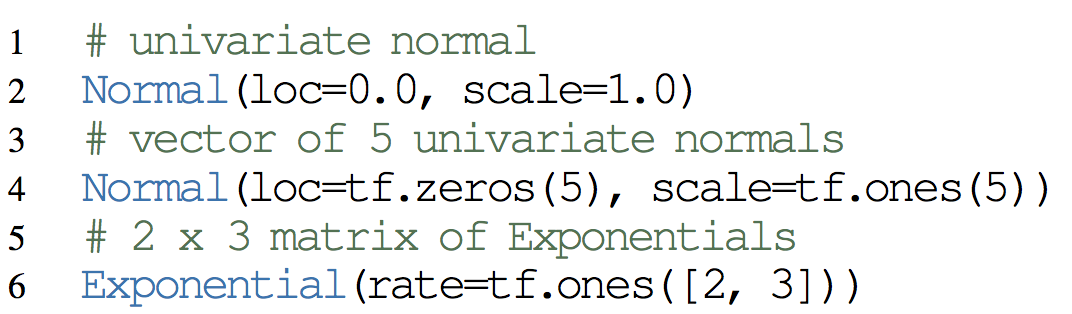
\includegraphics[height=0.20\textwidth]{img/random_variables.png}

Unlike \texttt{tf.Tensor}s, \texttt{ed.RandomVariable}s
carry an explicit density with methods
such as \texttt{log\_prob()} and \texttt{sample()}.

For implementation, we wrap all TensorFlow Distributions and call
\texttt{sample} to produce the associated tensor.
% Mutable states also let random variables condition on values that
% change, e.g., discriminative models $p(\mby\g\mbx)$ and model
% parameters $p(\mbx; \theta)$.
\end{frame}

\begin{frame}
\frametitle{Language Example}
\begin{center}
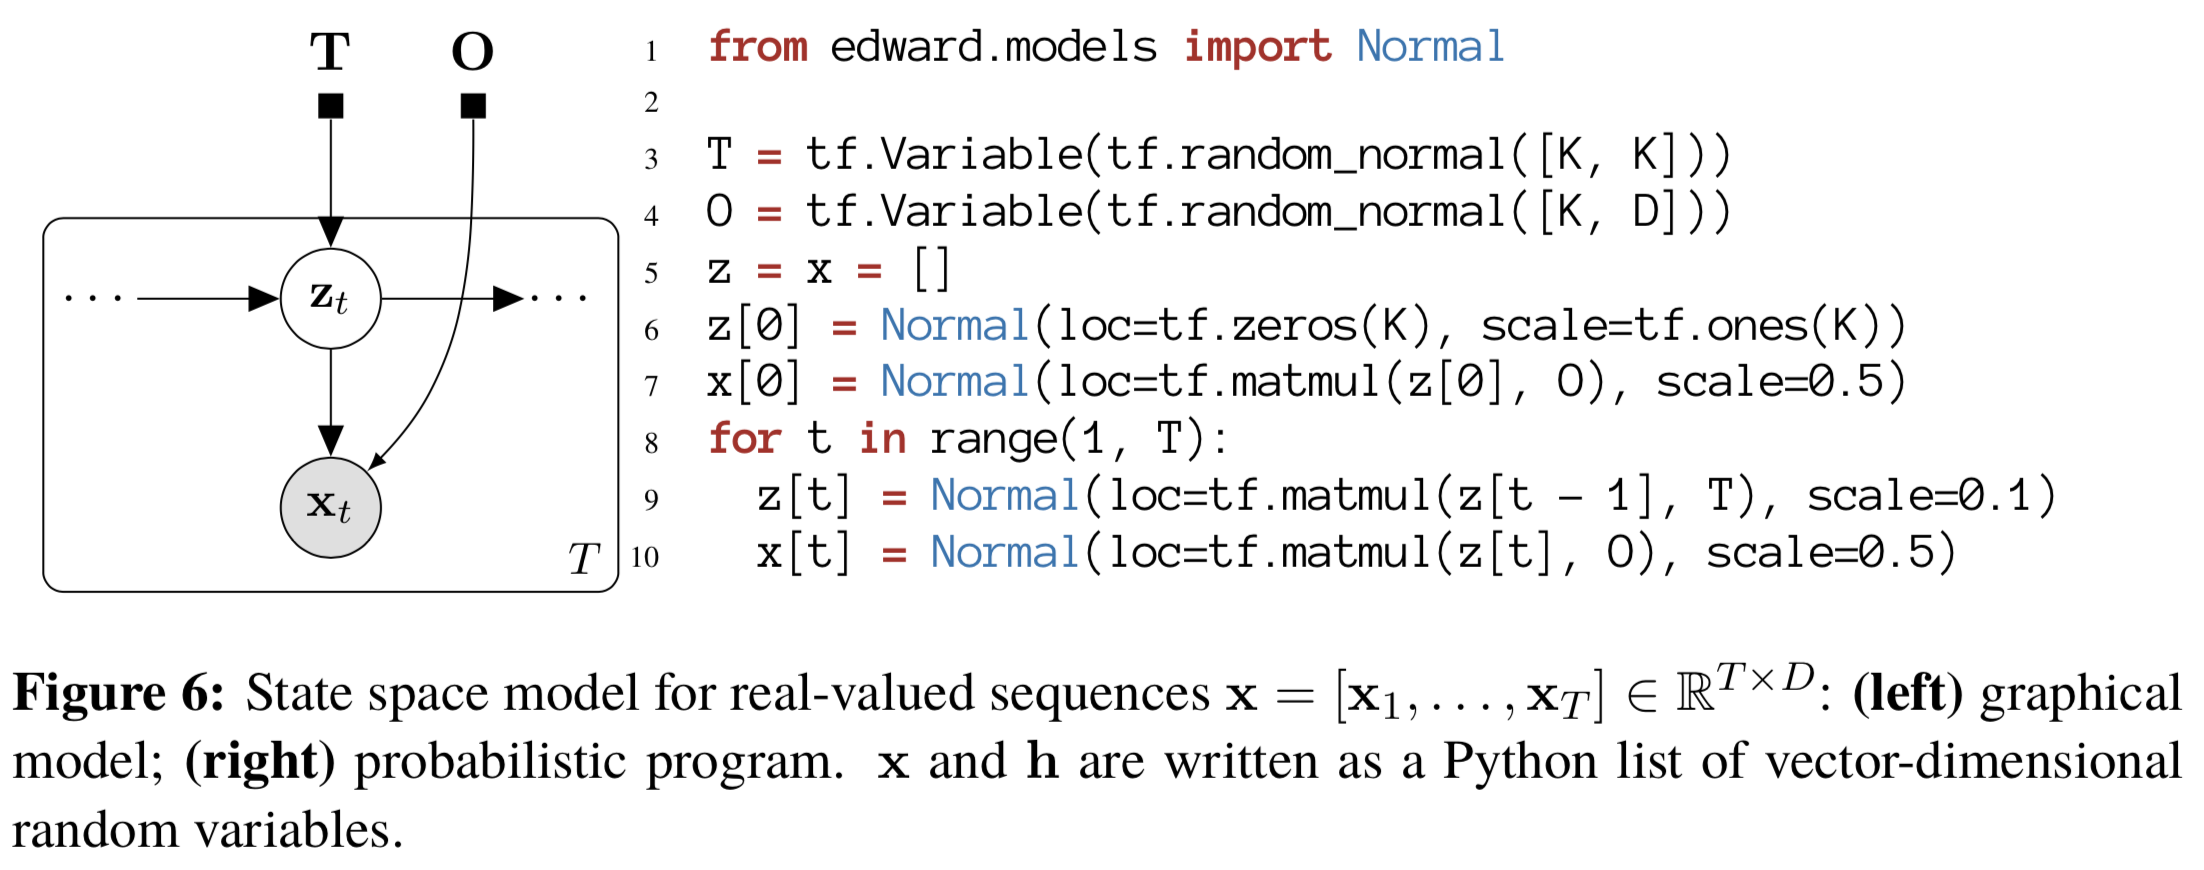
\includegraphics[width=1.05\textwidth]{img/ssm-program.png}
\end{center}

\vspace{1ex}
Edward's language enables a \emph{calculus} on random variables.
\end{frame}

% \begin{frame}
% \frametitle{Example: Bayesian neural network for classification}
% \begin{center}
% \includegraphics[height=0.3\textwidth]{img/bayesian_nn_graph.png}
% \\[2.5ex]
% \includegraphics[height=0.19\textwidth]{img/bayesian_nn_program.png}
% \end{center}
% \end{frame}

% \begin{frame}
% \frametitle{Example: Bayesian recurrent neural network}
% \begin{center}
% \includegraphics[height=0.32\textwidth]{img/bayesian_rnn_graph.png}
% 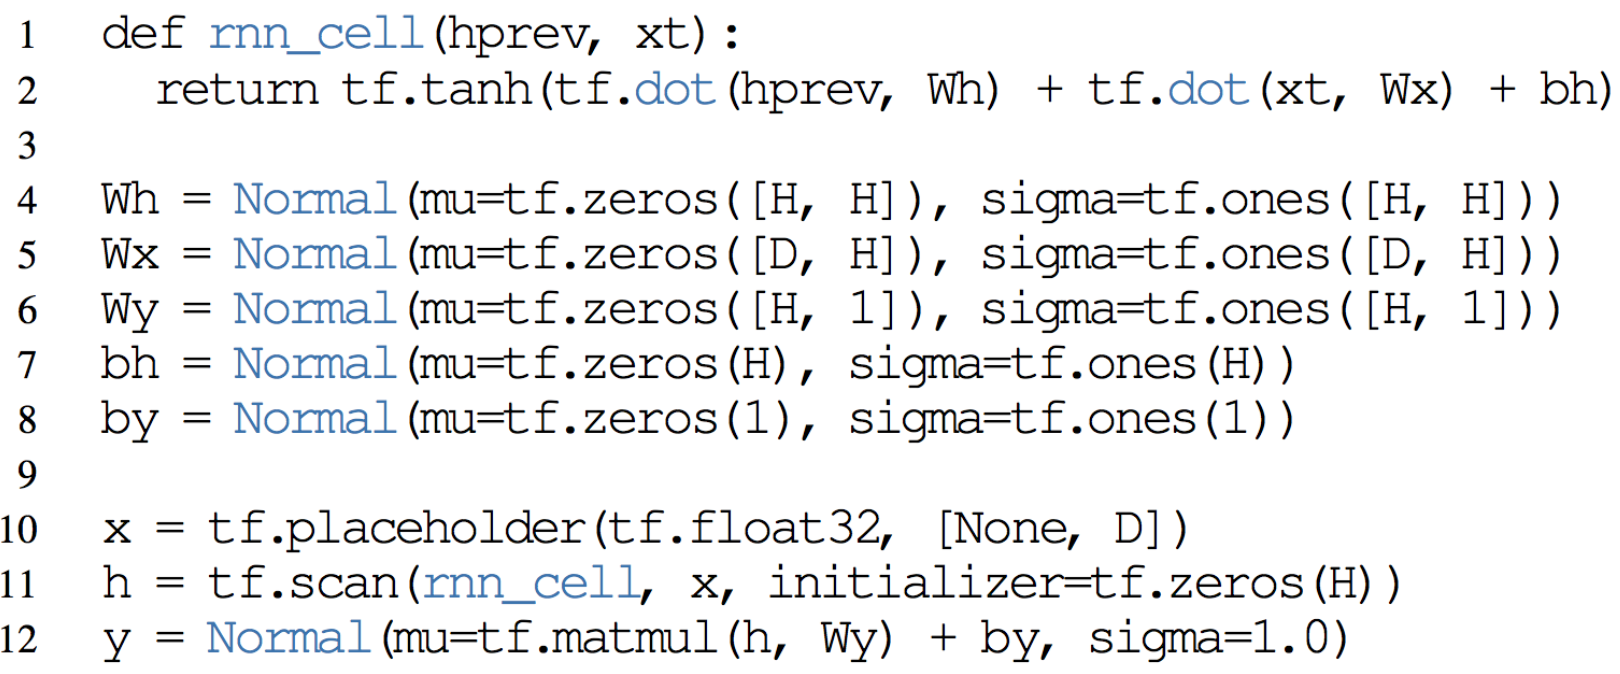
\includegraphics[height=0.32\textwidth]{img/bayesian_rnn_program.png}
% \end{center}
% \end{frame}

% \begin{frame}
% \frametitle{Example: Variational Auto-Encoder for Binarized MNIST}
% \begin{tikzpicture}[remember picture,overlay]
%   \node [xshift=0.4cm, yshift=-0.8cm, anchor=north west] at (current page.north west) {
%    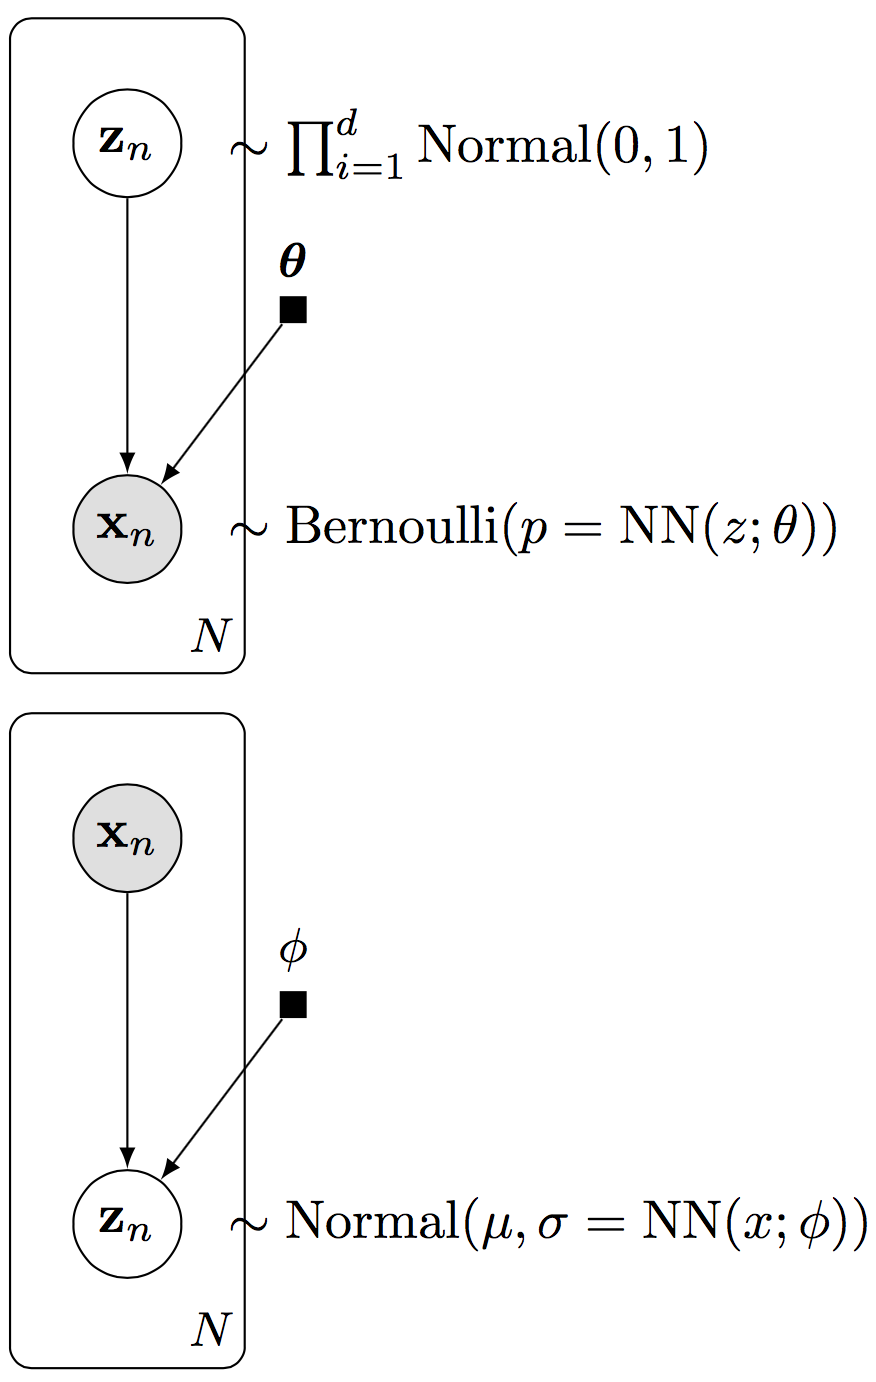
\includegraphics[width=0.5\columnwidth]{img/vae_graphical_model_01.png}
%   };
%   \node [xshift=-5.75cm, yshift=0.4cm, anchor=south west] at (current
%   page.south east) {
% \gray{\small [Kingma \& Welling 2014; Rezende+ 2014]}
%   };
% \end{tikzpicture}
% \end{frame}

% \begin{frame}
% \frametitle{Example: Variational Auto-Encoder for Binarized MNIST}
% \begin{tikzpicture}[remember picture,overlay]
%   \node [xshift=0.5cm, yshift=-1.0cm, anchor=north west] at (current page.north west) {
%    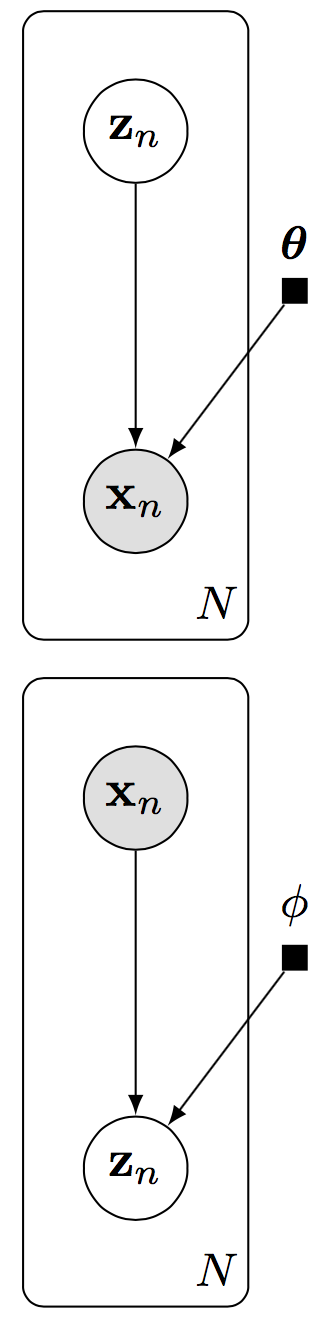
\includegraphics[width=0.18\columnwidth]{img/vae_graphical_model.png}
%   };
%   \node [xshift=2.6cm, yshift=-1.7cm, anchor=north west] at (current page.north west) {
% 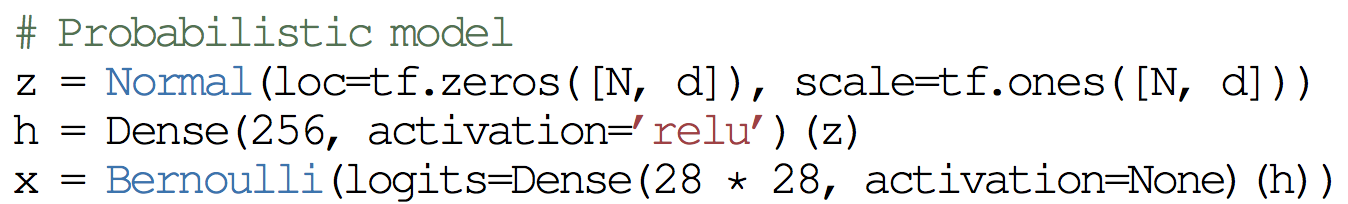
\includegraphics[height=0.14\textheight]{img/vae_decoder.png}
%   };
%   \node [xshift=2.6cm, yshift=-5.8cm, anchor=north west] at (current page.north west) {
% 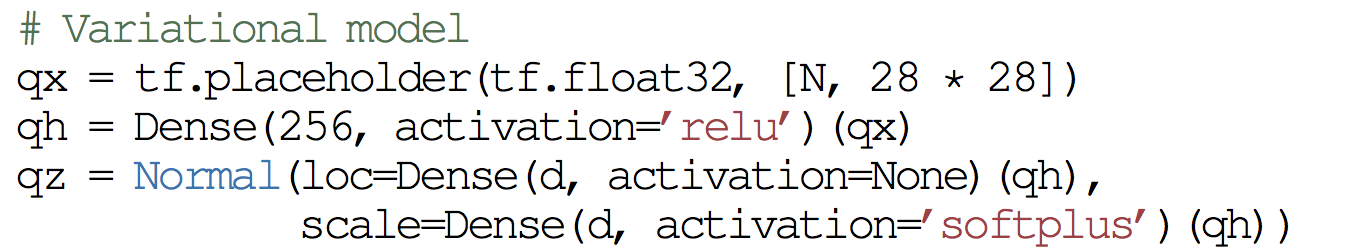
\includegraphics[height=0.18\textheight]{img/vae_encoder.png}
%   };
%   \node [xshift=-5.75cm, yshift=0.4cm, anchor=south west] at (current
%   page.south east) {
% \gray{\small [Kingma \& Welling 2014; Rezende+ 2014]}
%   };
% \end{tikzpicture}
% \end{frame}

% \begin{frame}
% \frametitle{Inference as Stochastic Graph Optimization}
% Given
% \begin{itemize}
% \item Data $\mbx_{\text{train}}$.
% \item
% Model $p(\mbx, \mbz, \mbbeta)$ of
% observed variables $\mbx$ and latent variables $\mbz, \mbbeta$.
% \end{itemize}
% Goal
% \begin{itemize}
% \item
% Calculate posterior distribution
% \begin{equation*}
% p(\mbz, \mbbeta\mid\mbx_{\text{train}}) =
% \frac{p(\mbx_{\text{train}}, \mbz, \mbbeta)}{\int
% p(\mbx_{\text{train}}, \mbz, \mbbeta) \d\mbz\d\mbbeta}.
% \end{equation*}
% \end{itemize}
% \vspace{2ex}
% This is the key problem in Bayesian inference.
% \begin{tikzpicture}[remember picture,overlay]
%   \node [xshift=-4.5cm, yshift=0.4cm, anchor=south west] at (current
%   page.south east) {
% \small \url{edwardlib.org/tutorials}
%   };
% \end{tikzpicture}
% \end{frame}

\begin{frame}
\frametitle{Inference as Stochastic Graph Optimization}

\begin{center}
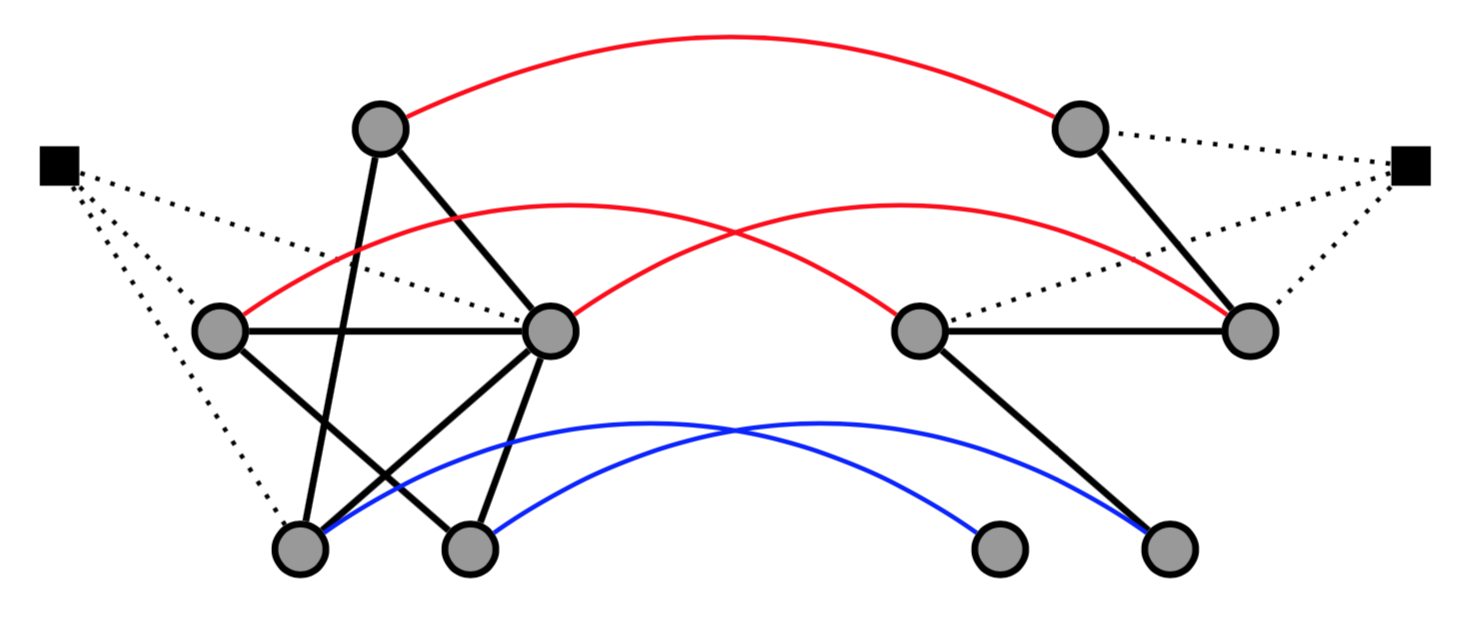
\includegraphics[width=0.7\textwidth]{img/inference-graph.png}
\end{center}

All \texttt{Inference} has (at least) two inputs: \\
\begin{enumerate}
\vspace{-3ex}
\item
\red{red} aligns latent variables and posterior approximations;
\item
\blue{blue} aligns observed variables and realizations.
\end{enumerate}

\begin{center}
\vspace{-2.0ex}
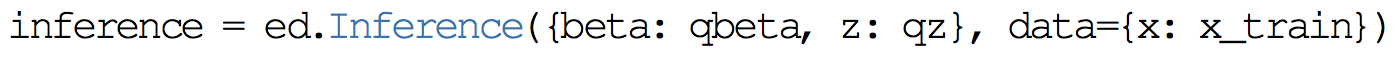
\includegraphics[height=0.05\textheight]{img/inference.png}
\end{center}

\texttt{Inference} has class methods to finely control the algorithm.
\end{frame}

\begin{frame}
\frametitle{Edward == handwritten TensorFlow at runtime}
\begin{center}
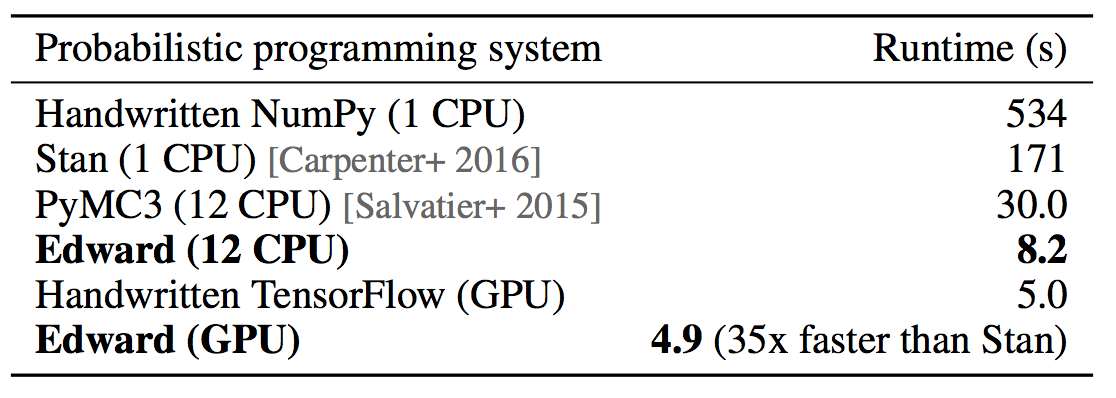
\includegraphics[width=0.85\textwidth]{img/experiments_hmc.png}
\end{center}
\vspace{-1ex}
Run HMC for 100 iterations and fixed hyperparameters.

Bayesian logistic regression for Covertype ($581012$ data points, $54$
features).

12-core Intel i7-5930K CPU at 3.50GHz and NVIDIA Titan X (Maxwell) GPU.
Single precision.

\vspace{4ex}
\textbf{Edward is orders of magnitude faster than existing software
for large data.}
\begin{tikzpicture}[remember picture,overlay]
  \node [xshift=-2cm, yshift=0.4cm, anchor=south west] at (current
  page.south east) {
\gray{\small [Tran+ 2017]}
  };
\end{tikzpicture}
\end{frame}

\begin{frame}
\frametitle{Composable \& Hybrid Inference}

\begin{center}
\vspace{-2ex}
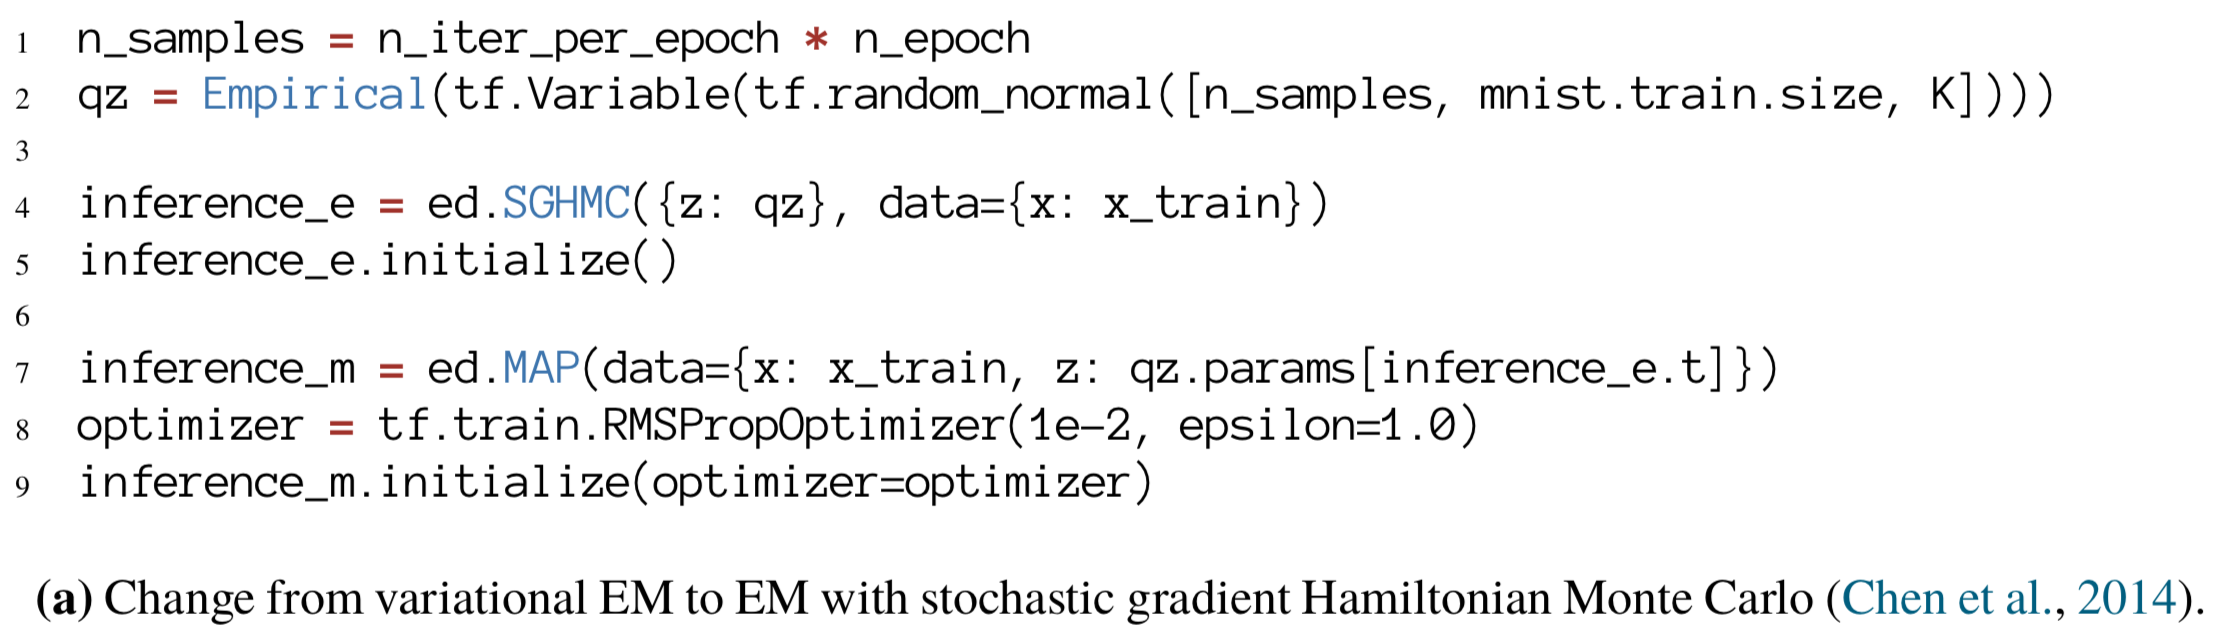
\includegraphics[width=1.0\textwidth]{img/em.png}
\vspace{2ex}

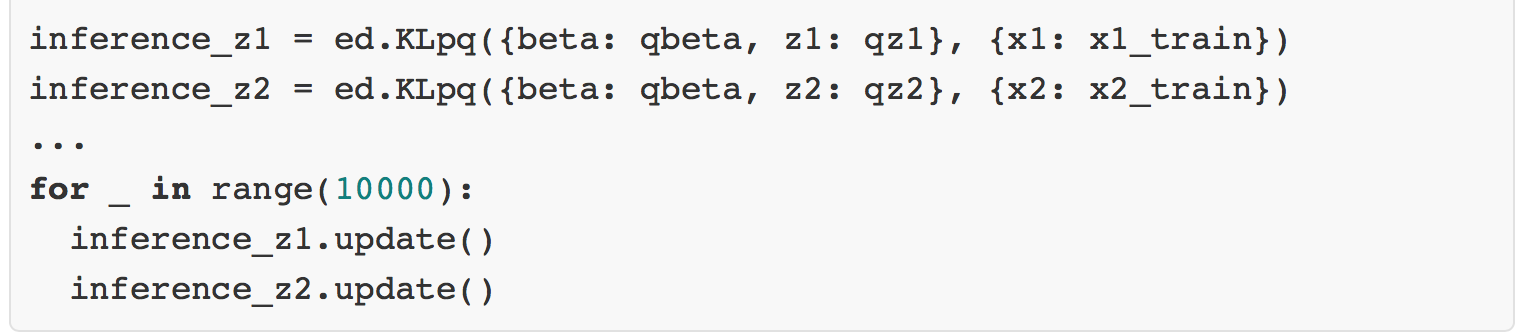
\includegraphics[width=1.0\textwidth]{img/ep.png}
% Composable inference (expectation propagation)
\end{center}

\begin{tikzpicture}[remember picture,overlay]
  \node [xshift=-8.0cm, yshift=0.4cm, anchor=south west] at (current
  page.south east) {
\small \url{edwardlib.org/api/inference-compositionality}
  };
\end{tikzpicture}
\end{frame}

\begin{frame}
\frametitle{Non-Bayesian Inference}
\begin{center}
\vspace{-2ex}
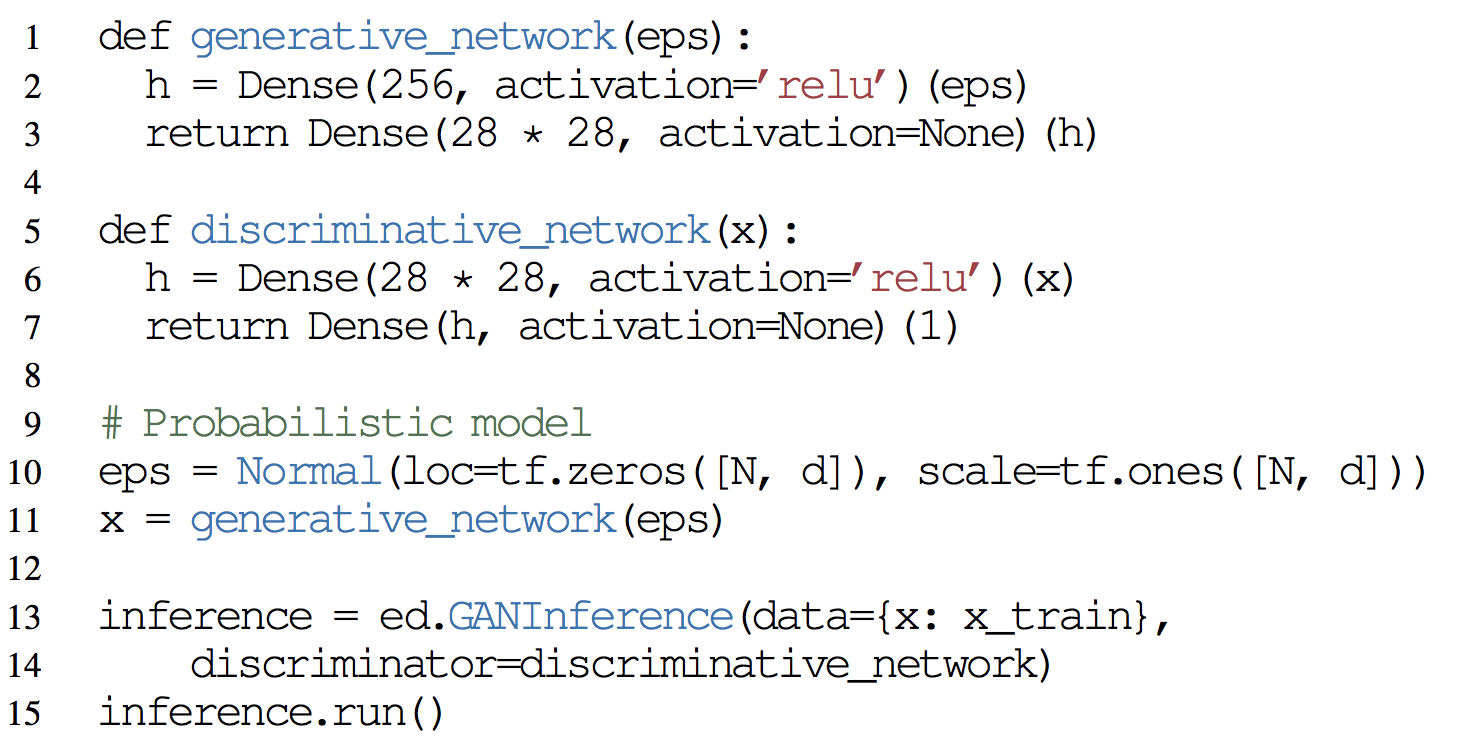
\includegraphics[width=1.0\textwidth]{img/gan_example.png}
\end{center}
\begin{tikzpicture}[remember picture,overlay]
  \node [xshift=-6.5cm, yshift=0.4cm, anchor=south west] at (current
  page.south east) {
\small \url{edwardlib.org/api/inference-classes}
  };
\end{tikzpicture}
\end{frame}

\begin{frame}
\begin{center}
{\Large\bf Some Cool Ideas}
\end{center}
\end{frame}

\begin{frame}
\frametitle{Against the ``Program -> Query'' Modality}
\begin{enumerate}
\item
Unlike other PPLs, \textbf{Edward has no explicit ``model'' or ``inference''
block}: \\
A model is simply a collection of random variables in the graph.  \\
Inference specifies how to modify parameters in that
collection subject to another.

This offers significant flexibility: we can
% With conditional inference,
% we can simultaneously run updates over multiple algorithms like
% \Cref{fig:alignment} but over different alignments.
\emph{infer only parts of a model} (e.g.,
layer-wise training),
\emph{infer parts used in multiple models}
(e.g., multi-task learning), or
\emph{plug in a posterior into a new model}
(e.g., Bayesian updating).
\item
Unlike other PPLs, \textbf{Edward has no \texttt{observe} operator}, which is called
before an \texttt{infer} operation.
% unlike church-like langs which use a condition/observe operator, pymc3, stan compilation, and even modern ppls like pyro
% random variables are not tied to observations.
Each \texttt{Inference} can specify its own alignment of random
variables and observations.
\end{enumerate}
\end{frame}

\begin{frame}[plain,t]
\frametitle{Implicit Models (\& Likelihood-Free Inference)}
\begin{center}
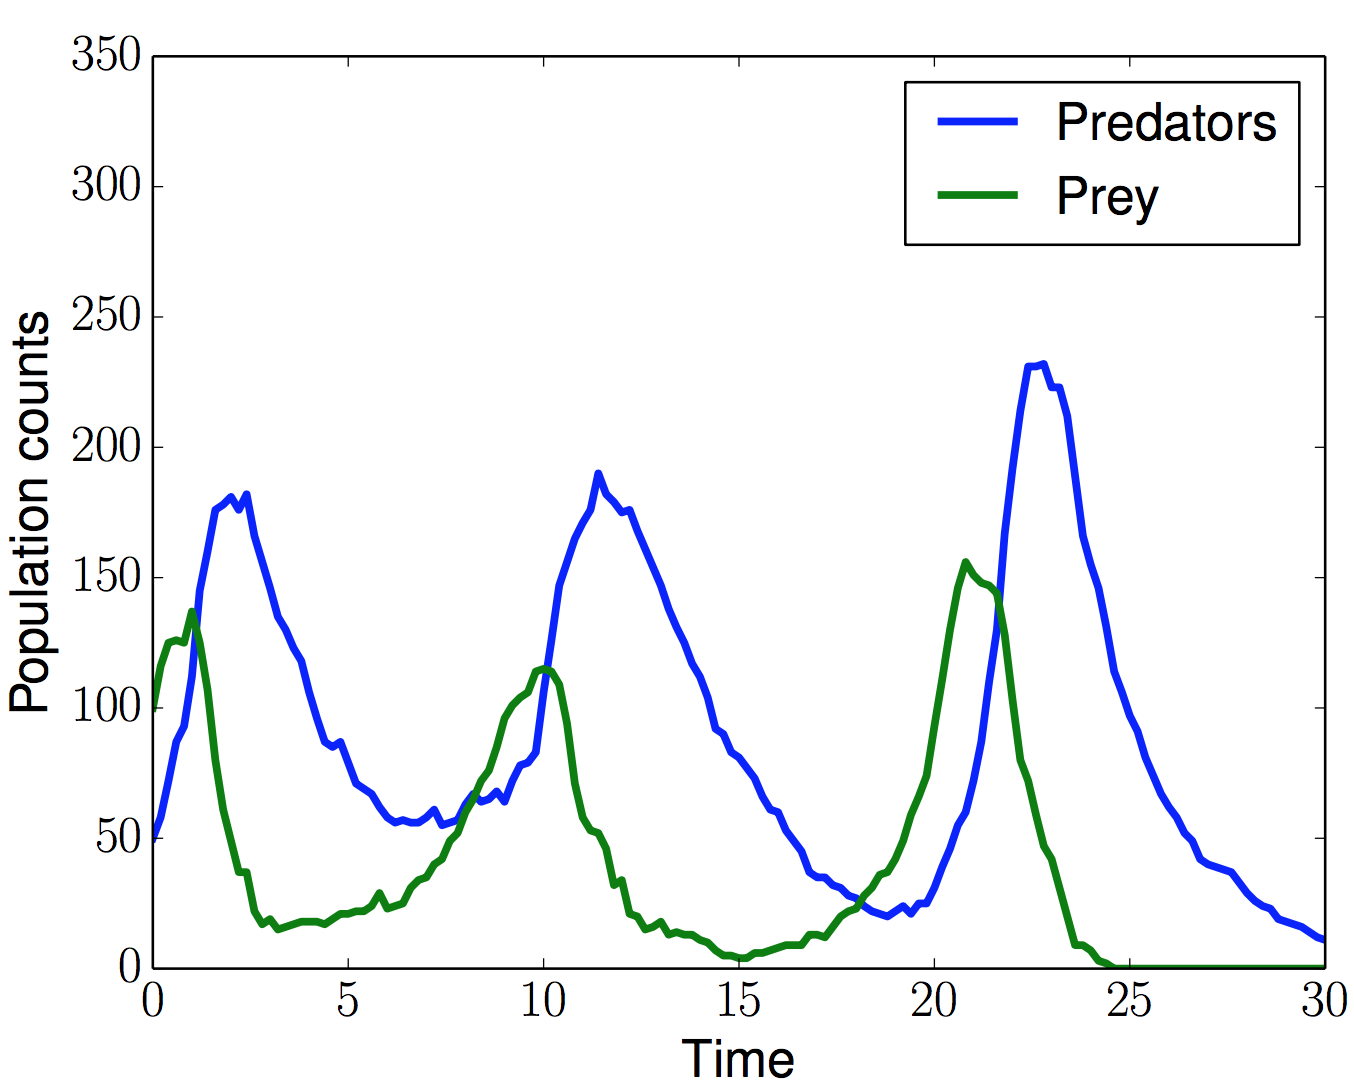
\includegraphics[width=0.6\textwidth]{img/lotka_volterra_plot.png}
\end{center}

\begin{center}
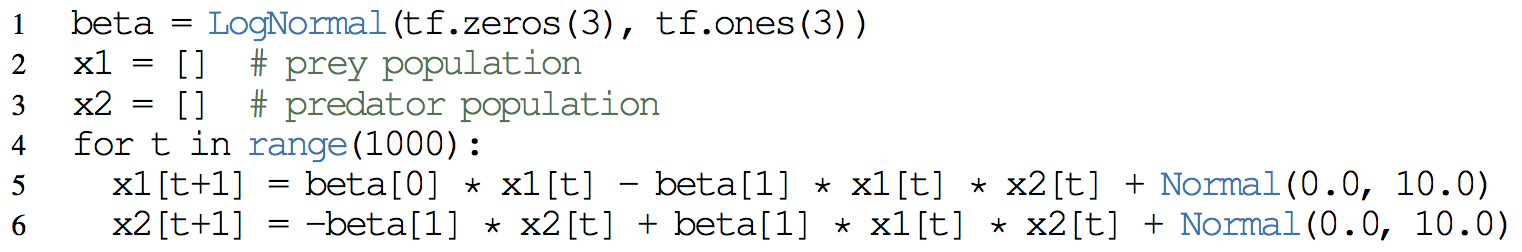
\includegraphics[width=1.0\textwidth]{img/lotka_volterra_program.png}
\end{center}
\texttt{tf.Tensors} implicitly carry densities. We can infer (approximate)
them via \texttt{Inference}.
\end{frame}

\begin{frame}
\frametitle{Dynamic Stochasticity}
Parameter shapes can be stochastic.

\begin{center}
\hspace{-11em}
\vspace{-1.0ex}
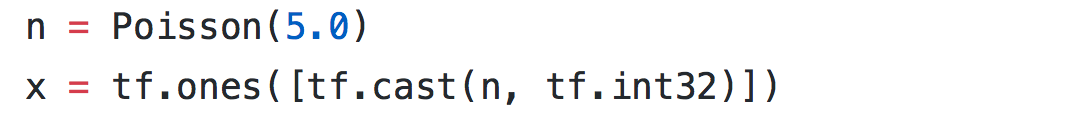
\includegraphics[width=0.7\textwidth]{img/poisson.png}
\end{center}

Event shapes can be stochastic.

\begin{center}
\vspace{-0.5ex}
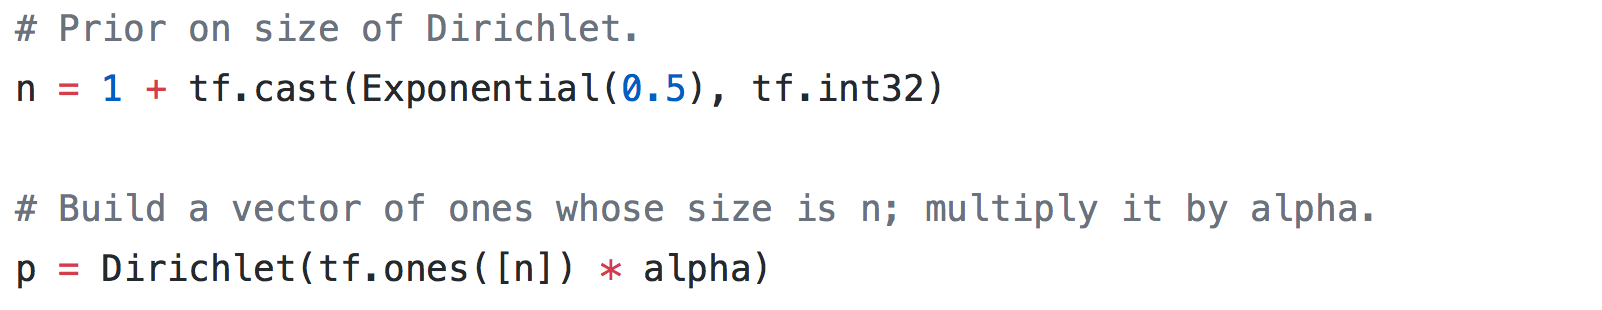
\includegraphics[width=1.0\textwidth]{img/dirichlet.png}
\vspace{-2ex}
\end{center}

Control flow can be stochastic.

\begin{center}
\vspace{-0.5ex}
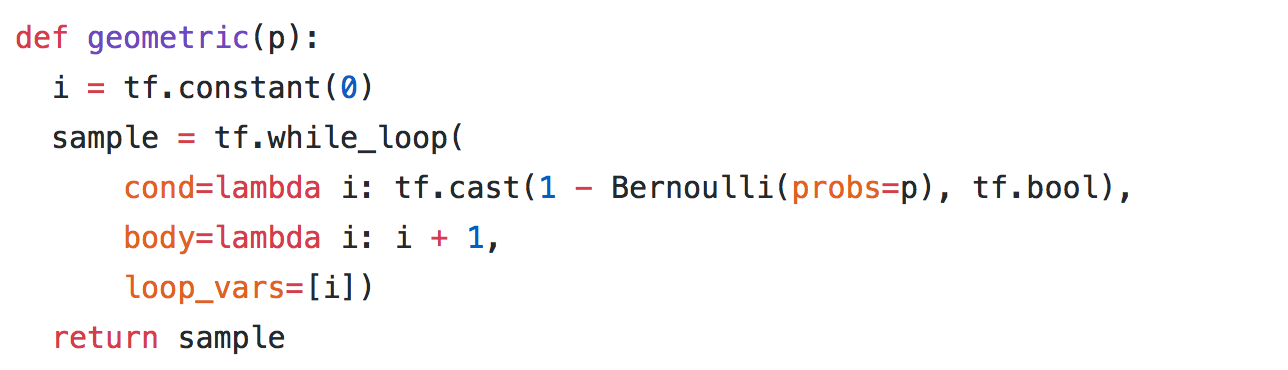
\includegraphics[width=1.0\textwidth]{img/geometric.png}
\vspace{-2ex}
\end{center}

No recursion. Must be rewritten as a (stochastic) while loop.
We implemented a DirichletProcess this way.
% + no recursion; must express via while loop
\end{frame}

\begin{frame}
\frametitle{Taxonomy of Inference}
\begin{center}
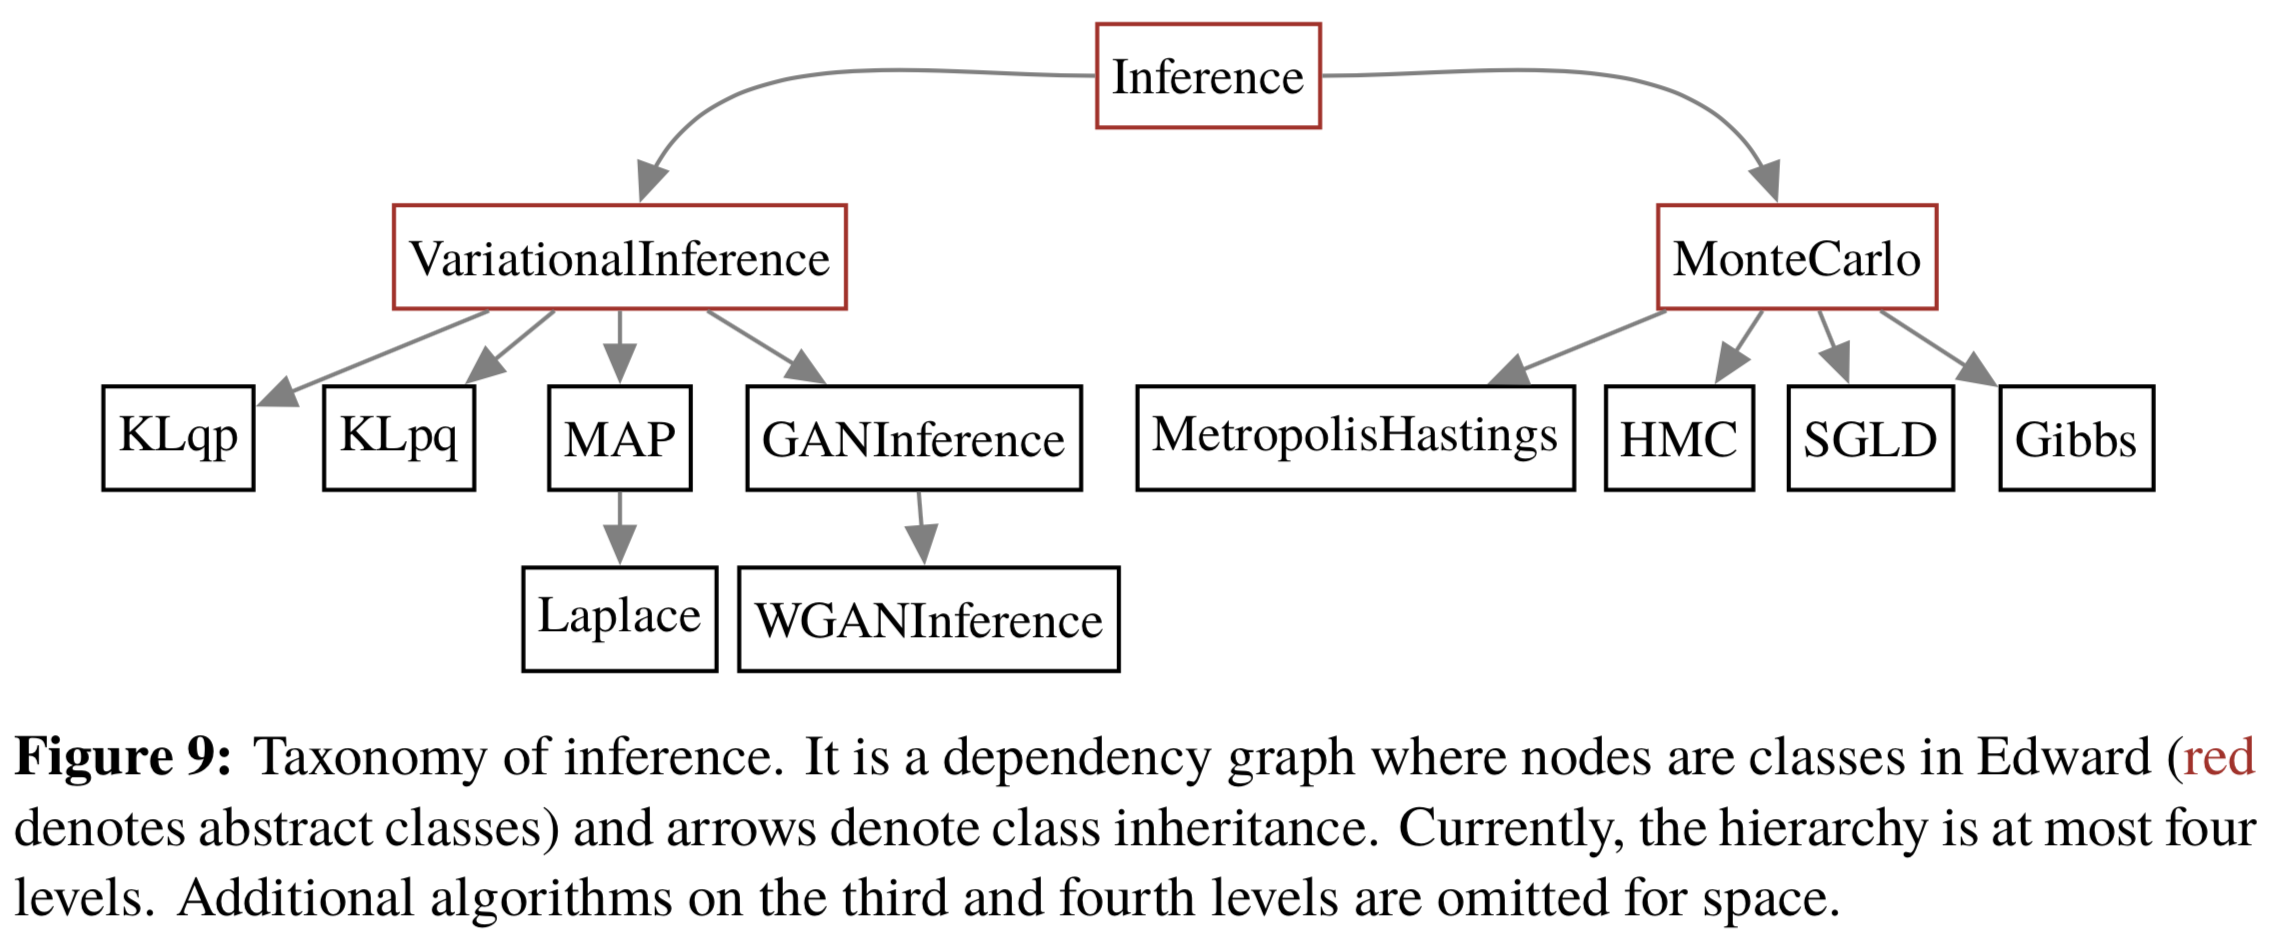
\includegraphics[width=1.0\textwidth]{img/taxonomy.png}
\end{center}
\end{frame}

\begin{frame}
\frametitle{Compiler Connections}
Recall Edward interprets inference as stochastic graph optimization.

This may have deep implication to extend compiler optimization with
probability(?).
Examples:
\begin{enumerate}
\item
\textbf{Operation fusion to marginalization.}
% GPU kernels are memory-bound. Fusing kernels allows kernels
% to share data and reduce traffic to off-chip memory.
% The equivalent operation for two stochastic kernels is
% marginalization.
Fusing two stochastic nodes into one corresponds to computing the
marginal density.
(E.g., turn naive Monte Carlo sample to exact normal-normal compound density.)
\item
\textbf{Common subexpression elimination to common distribution
elimination.}
Suppose a graph involves compiling two subgraphs which
are approximately equal in distributions. Avoid compiling them
separately.
\item
\textbf{Amortized inference as ahead-of-time compilation.}
Training can amortize inference over data generated from the model; no
data need be involved until runtime.
\end{enumerate}
These are half-baked, experimental ideas. Worth more investigation.
\end{frame}

\begin{frame}
\frametitle{Exploiting Graphs: Conditional Independence}

\begin{center}
\vspace{-2ex}
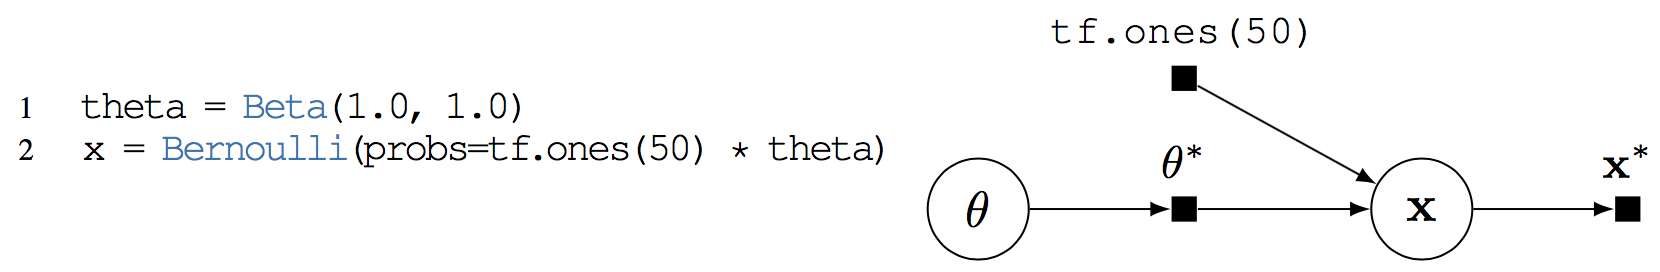
\includegraphics[height=0.175\textwidth]{img/beta-bernoulli.png}
\end{center}

Edward writes all programs as part of the computational graph.
This lets us exploit graph structure.
One powerful application is conditional independence.

\begin{itemize}
\item
Edward can query a random variable for its parents,
ancestors, children, and Markov blanket.
\item
Edward uses Bayes-Ball to assess conditional independence of two
nodes given a third set of nodes.
\item
Operators for causal graphs (e.g., backdoor criterion) are also
possible.
\end{itemize}
Why is this important? Conditional independence is fundamental to
distributed inference by enabling parallel, concurrent computation.
% Fetching $\mbx$ from the graph generates a binary vector of $50$ elements.
\end{frame}

\begin{frame}
\frametitle{Exploiting Graphs: Symbolic Algebra}
We can exploit graphs not just in the graph structure but in the
symbolic operations.

This enables a \texttt{complete\_conditional} function. Basically it:
\begin{enumerate}
\item
Take a random variable's Markov blanket; then take the log joint.
\item
Simplify the log joint into a set of sufficient statistic and natural
parameter pairs.
\item
Perform a table lookup to find the distribution corresponding to those
sufficient statistics.
\end{enumerate}

Why is this important?
It is core to Edward's \texttt{Gibbs} and VI with natural gradients.
\end{frame}

% \begin{frame}
% \frametitle{Ongoing Directions}

% We are extending Edward's design.
% \begin{enumerate}
% \item
% Integration with a probabilistic intermediate representation
% (BayesFlow).
% \item
% TPUs \& XLA.
% \item
% Distributed probabilistic programming.
% % \item
% % A one-line API for loading standard data sets in machine learning.
% \end{enumerate}
% \vspace{3ex}

% We are applying Edward for AI and scientific research.
% \begin{enumerate}
% \item
% Causal models for genome wide association studies.
% \item
% Alignment \& semi-supervised learning in text.
% \end{enumerate}
% \end{frame}

% \begin{frame}[t]
% \frametitle{Example: Variational Auto-Encoder for Binarized MNIST}
% \vspace{5ex}
% \begin{center}
% 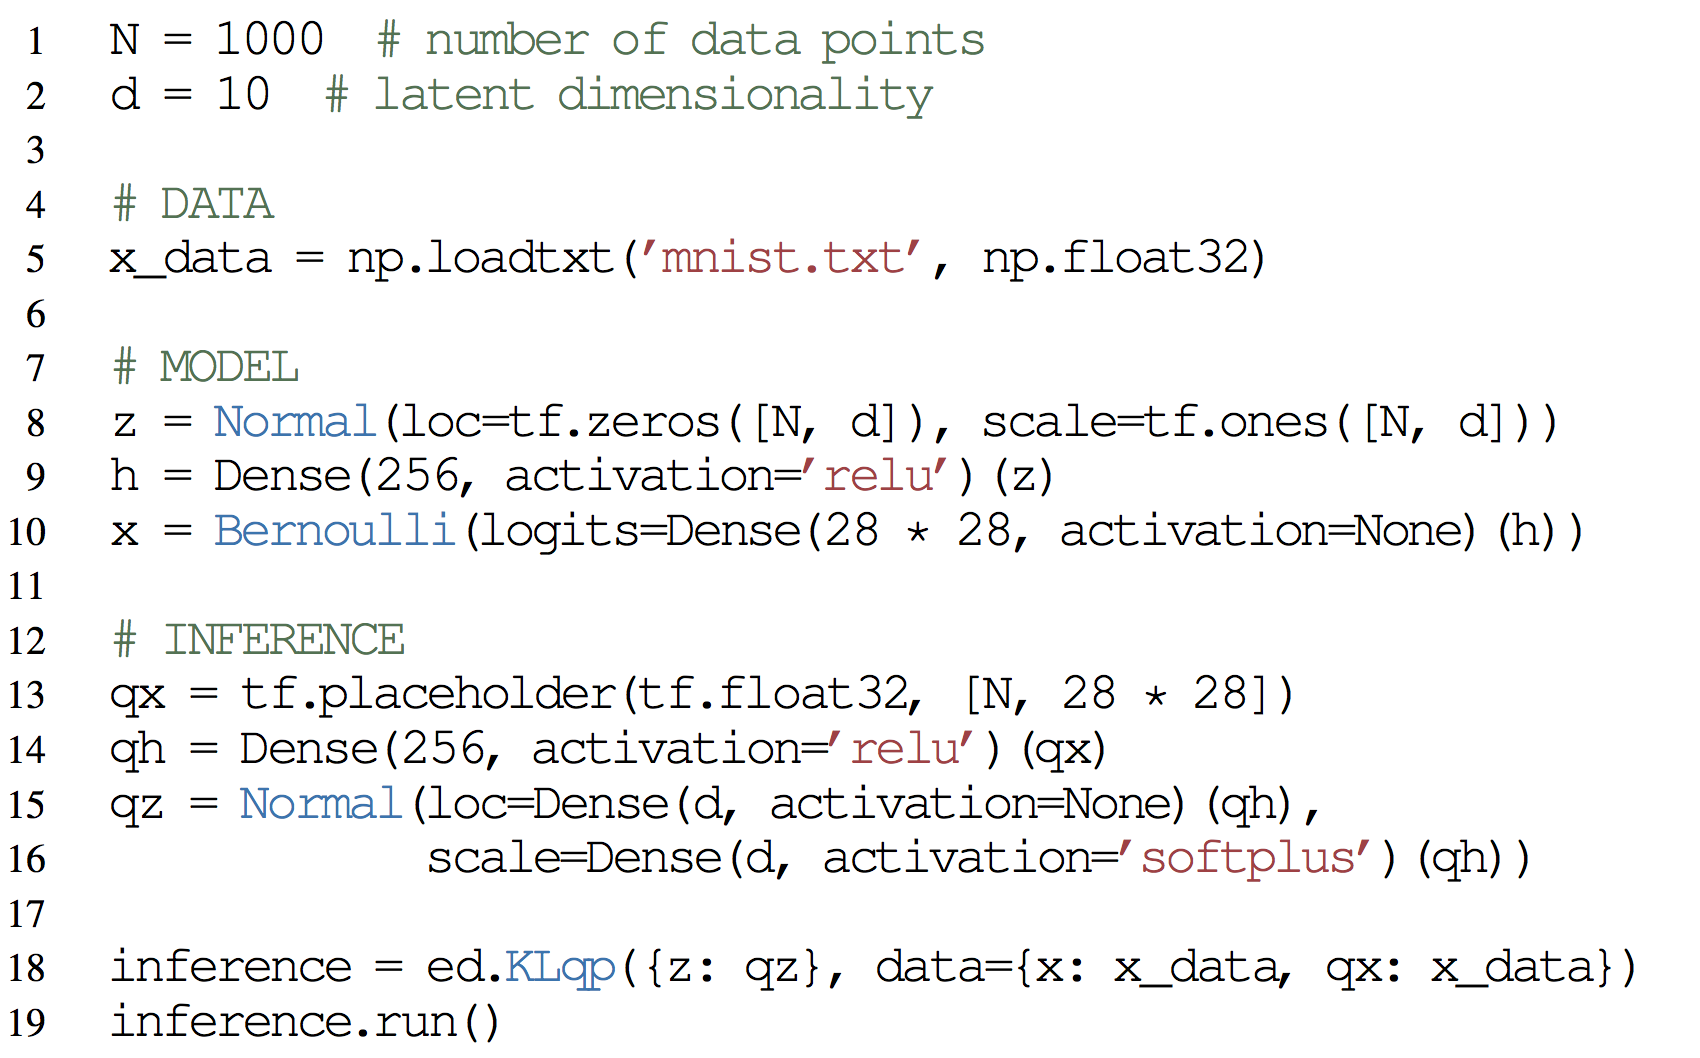
\includegraphics[width=0.975\textwidth]{img/vae_example.png}
% \end{center}
% \end{frame}

% \begin{frame}[t]
% \frametitle{Example: Variational Auto-Encoder for Binarized MNIST}
% \vspace{2.5ex}
% \begin{center}
% 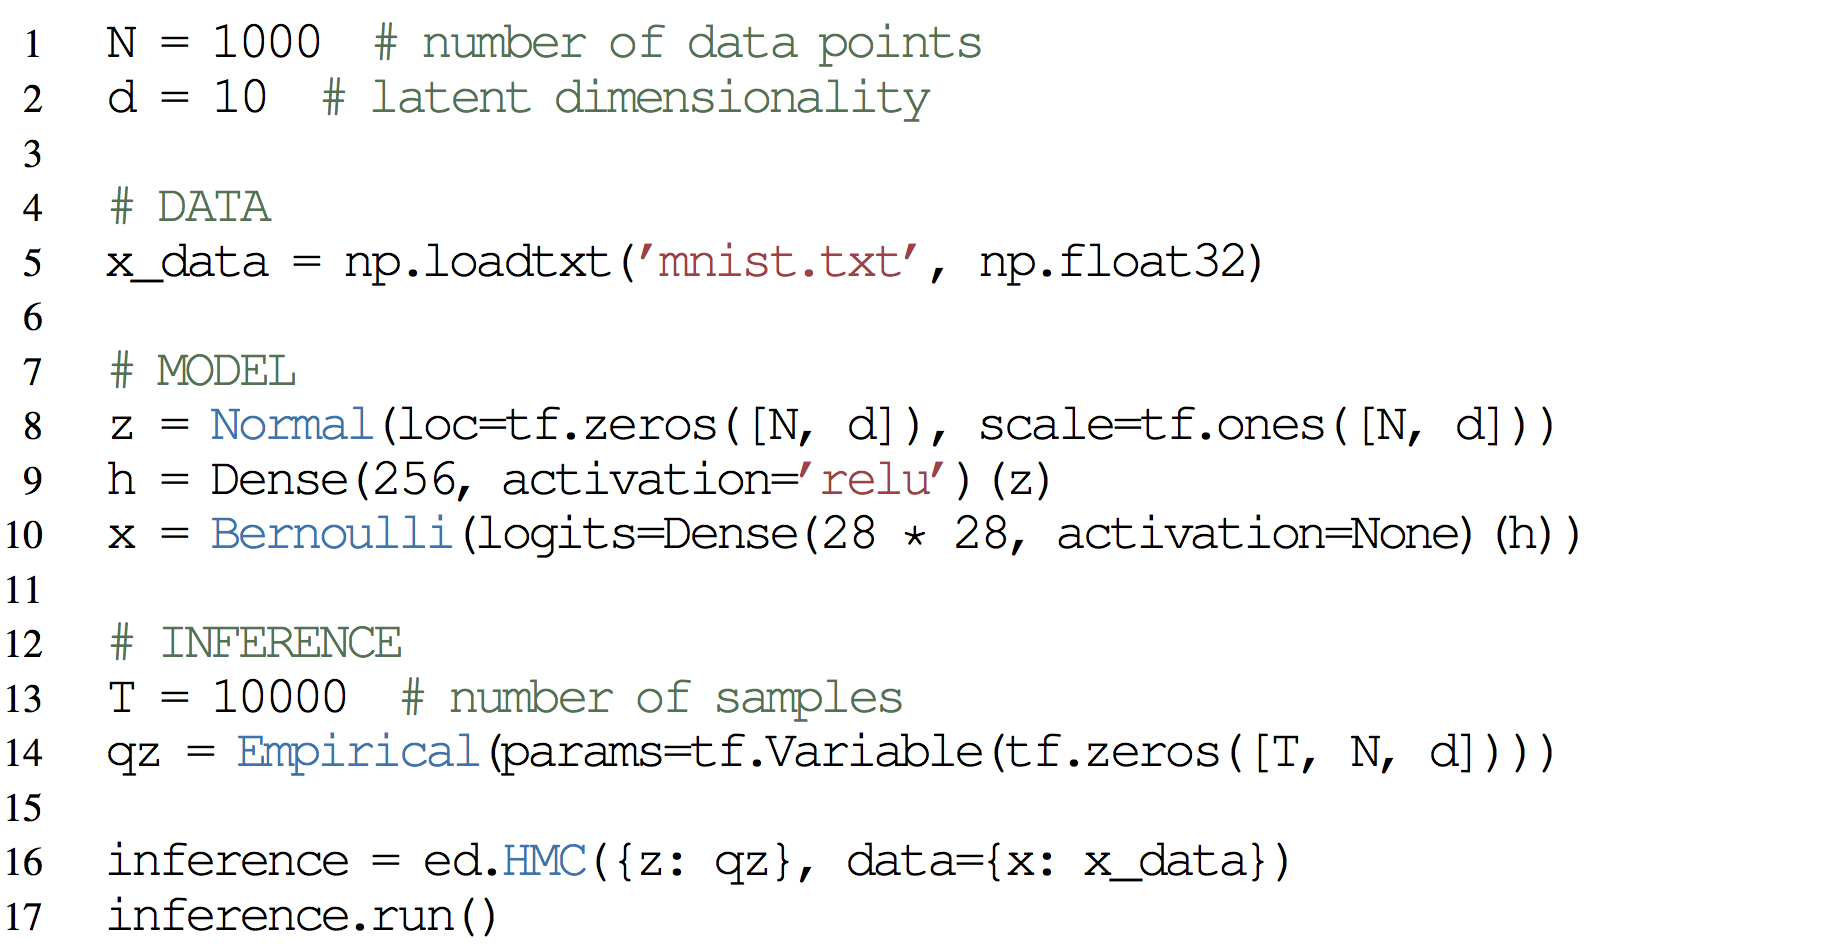
\includegraphics[width=1.05\textwidth]{img/vae_example_hmc.png}
% \end{center}
% \end{frame}

\begin{frame}
\frametitle{Limitations}
\begin{itemize}
\item
\textbf{Graph copying} is a key function to all Edward's inferences. It's a
cognitive PITA, carries graph junk, and hides computation from users.
% \item
% + can't get more fine-grained detail for single node operations, e.g.,
% rao-blackwellization, EP when representing one RV node for batch
\item
\textbf{Object-oriented inference} has a high cognitive burden. Arguably no one
except me understands it enough to exploit.
\item
Certain models, such as autoregressive distributions, are easier to
\textbf{build the loss} (log prob) than it is to build the generative program.
\item
\textbf{Programmable inference is hard}. Matt and I thought hard about
use cases. But we didn't cover all of them. Ex: gradient clipping,
registering specific inference ops to devices.
\end{itemize}
\end{frame}

\begin{frame}
\frametitle{Questions}
\begin{itemize}
\item
Edward's biggest competitor is not an existing PPL, but TensorFlow itself.
% Integration with a probabilistic intermediate representation
% (BayesFlow).
% \red{How do we refactor Edward to use our new
% intermediate representation?}

% \red{Rather than start from statistics where computation is induced
% by statistical queries, can we start from the bottom-up
% (``computation-first'')?}
\red{Rather than start from universal PPLs and bend backwards to
support programmable inference, can we take a
\textbf{computation-first}
approach?}
% \item
% \red{How can Edward support TPUs \& XLA?}
\item
Edward is limited to single machine.

\red{How do we scale probabilistic programming to
\textbf{multi-machine}
environments with billions of data points?}
\item
Our \textbf{symbolic algebra} works on only toy problems and requires
TensorFlow graph introspection.

\red{Can we pursue this at the XLA graph level?}
\item
Our ICLR paper proposed a \textbf{model zoo}. The idea is to
go beyond Stan's model examples to also include
inference algs, tuned hyperparameters, and pre-training.
It never took off.

\red{How do we make it usable?}
\end{itemize}
\end{frame}

\end{document}
